% Created 2016-05-16 Mon 02:22

\documentclass[14pt, a4paper]{extreport}

\newcommand{\comment}[1]{}

\usepackage{hyperref}
\usepackage{graphicx}
\usepackage[utf8]{inputenc}
\usepackage[T1,T2A]{fontenc}
\usepackage{textcase}
\usepackage{fixltx2e}
\usepackage{grffile}
\usepackage{longtable}
\usepackage{wrapfig}
\usepackage{rotating}
\usepackage[normalem]{ulem}
\usepackage{amsmath}
\usepackage{textcomp}
\usepackage{amssymb}
\usepackage{capt-of}
\usepackage{listings}
\usepackage{totcount}
\usepackage[figure,table]{totalcount}
\usepackage{etoolbox}
\usepackage{tocvsec2}
\usepackage{booktabs}

\graphicspath{ {./images/} }

\renewcommand*{\lstlistingname}{Листинг}

\lstset{
	numbers=left, 
	numberstyle=\small, 
	numbersep=8pt, 
	frame = single,
	framexleftmargin=0pt,
	breaklines=true,
	tabsize=2,
	showspaces=false,
	captionpos=b,
	showstringspaces=false
}

\setcounter{secnumdepth}{2}

\regtotcounter{page}

\newtotcounter{citenum}
\def\oldcite{}
\let\oldcite=\bibcite
\def\bibcite{\stepcounter{citenum}\oldcite}

\newtotcounter{attachcnt}

\usepackage{indentfirst}
\usepackage[left=3cm,right=1cm,
  top=2cm,bottom=2cm,bindingoffset=0cm]{geometry}
\usepackage[nodisplayskipstretch]{setspace}
\onehalfspacing
\sloppy
%\parindent=1cm

\usepackage{enumitem}
\setlist{nolistsep}

\usepackage{titlesec}
\titleformat{\chapter}[display]{\filcenter\bfseries\Large}{}{8pt}{}{}
\titleformat{\section}{\bfseries\Large}{\thesection}{1em}{}{}
\titleformat{\subsection}{\bfseries\normalsize}{\thesubsection}{1em}{}{}
\titleformat{\subsubsection}{\bfseries\normalsize}{}{1em}{}{}

% Настройка вертикальных и горизонтальных отступов
\titlespacing*{\chapter}{0pt}{-30pt}{*2}
\titlespacing*{\section}{\parindent}{*2}{*1}
\titlespacing*{\subsection}{\parindent}{*2}{*1}
\titlespacing*{\subsubsection}{\parindent}{*0.5}{*0}

\usepackage{polyglossia}
\setdefaultlanguage[spelling=modern]{russian}
\setotherlanguage{english}
\defaultfontfeatures{Mapping=tex-text}
\newfontfamily{\cyrillicfont}{Times New Roman}
\newfontfamily{\cyrillicfonttt}{Courier New} % шрифт URL-ссылок
%\newfontfamily{\sourcecodefont}{Courier New}
\defaultfontfeatures{Ligatures={TeX},Renderer=Basic}    %% свойства шрифтов по умолчанию
\setmainfont[Ligatures={TeX,Historic}]{Times New Roman} %% задаёт основной шрифт документа
%% \setsansfont{CMU Sans Serif}                         %% задаёт шрифт без засечек
\setmonofont{Courier New}                               %% задаёт моноширинный шрифт

\newcommand{\fixedspaceword}[2][1]{%
  \begingroup
  \spaceskip=#1\fontdimen2\font
  \xspaceskip=0pt\relax % just to be sure
  #2%
  \endgroup
}

% объявляем новую команду для переноса строки внутри ячейки таблицы
\newcommand{\spcell}[2][c]{%
  \begin{tabular}[#1]{@{}c@{}}#2\end{tabular}}

\bibliographystyle{gost705}

\makeatletter
\def\@biblabel#1{#1. }
\makeatother

\usepackage{caption}
\AtBeginDocument{%
  \def\contentsname{ОГЛАВЛЕНИЕ}
  \def\bibname{СПИСОК ИСПОЛЬЗОВАННОЙ ЛИТЕРАТУРЫ}
  \renewcommand{\figurename}{Рисунок}
  \renewcommand{\tablename}{Таблица}
  \renewcommand{\thefigure}{\arabic{chapter}.\arabic{figure}}
  \renewcommand{\thetable}{\arabic{chapter}.\arabic{table}}
  \renewcommand{\theequation}{\arabic{chapter}.\arabic{equation}}
}

\hypersetup{
  pdfauthor={Карасик С.Б.},
  pdftitle={Методы написания дипломной работы в последний момент перед предзащитой},
  pdfkeywords={СПИСОК КЛЮЧЕВЫХ СЛОВ, КАСАЮЩИХСЯ ТЕМЫ РАБОТЫ},
  pdfsubject={Тема работы},
  pdfcreator={xelatex},
  pdflang={Russian}
}


\gdef\goodbreak{\par\penalty-500}
\renewcommand\appendixname{Приложение}
\gdef\appendix{
	\par
	\setcounter{section}{0}
	\setcounter{subsection}{0}
	\def\thesection{\Asbuk{section}}
	\def\section##1{
		\refstepcounter{section}

		\begin{center}
			\goodbreak\noindent{
				\indent\Large\bf\hbox to 8.5em{\MakeTextUppercase{\appendixname}\ \thesection\hss}
				\nobreak\vspace{1em}\nobreak\noindent
				\linebreak
				##1
			}
		\end{center}
		\addcontentsline{toc}{chapter}{\hbox to 8.5em{\appendixname\ \thesection\hss}\hspace{0.8ex}##1}
	}
}


\begin{document}

%%% начало документа
%%% заглушка титульного листа, настоящий делать на основе образца в файле Titul.doc

% \maketitle
\begin{titlepage}
	\begin{center}
		\large
		МИНИСТЕРСТВО ОБРАЗОВАНИЯ РЕСПУБЛИКИ БЕЛАРУСЬ
		
		\vspace{0.5cm}
		
		БЕЛОРУССКИЙ ГОСУДАРСТВЕННЫЙ УНИВЕРСИТЕТ
		\vspace{0.5cm}
		
		ФАКУЛЬТЕТ ПРИКЛАДНОЙ МАТЕМАТИКИ И ИНФОРМАТИКИ
		
		\vspace{0.25cm}
		
		Кафедра математического моделирования и анализа данных
		\vfill
		
		{\LARGE ПОСТРОЕНИЕ ОПТИМАЛЬНЫХ ПЛАНОВ ЭКСПЕРИМЕНТА ДЛЯ ЛИНЕЙНОЙ МНОЖЕСТВЕННОЙ РЕГРЕССИИ С ГЕТЕРОСКЕДАСТИЧЕСКИМИ  НАБЛЮДЕНИЯМИ}
		\bigskip
		
		\textsc{Отчёт по преддипломной практике}\\
	\end{center}
	\vfill
	
	\newlength{\ML}
	\settowidth{\ML}{«\underline{\hspace{0.7cm}}» \underline{\hspace{2cm}}}
	\hfill\begin{minipage}{0.5\textwidth}
		Карасика Семёна Борисовича\\
		студента 4 курса,\\
		специальность\\
		«прикладная математика»\\
	\end{minipage}%
	\bigskip
	
	\hfill\begin{minipage}{0.5\textwidth}
		Научный руководитель:\\
		кандидат физико-математических наук, доцент\\В.П. Кирлица
	\end{minipage}%
	\vfill
	
	\begin{center}
		Минск, 2020 г.
	\end{center}
\end{titlepage}

%%% описание рефератов

\setcounter{page}{2}

\settocdepth{chapter}

% \chapter*{РЕФЕРАТ}
% Дипломная работа: \total{page}\ страниц, \totalfigures{}~иллюстраций, \totaltables{}\ таблиц,
\total{citenum}\ источников, 5 приложений.

\vspace{\baselineskip}

ТОЧНЫЕ $D$-ОПТИМАЛЬНЫЕ ПЛАНЫ ЭКСПЕРИМЕНТОВ, ЛИНЕЙНАЯ МНОЖЕСТВЕННАЯ РЕГРЕССИЯ, НЕРАВНОТОЧНЫЕ НАБЛЮДЕНИЯ.

\vspace{\baselineskip}

Объект исследования – неравноточные наблюдения. Цель работы – разработать методы построения $D$-оптимальных планов экспериментов для неравноточных наблюдений.

Методы исследования – методы теории вероятностей, математической
статистики, теория оптимального эксперимента.

Результатами являются построенные $D$-оптимальные планы для неравноточных наблюдений с 2 и 3 независимыми переменными, с линейным изменением.

Областью применения являются планирование научных и производственных экспериментов.


% \chapter*{РЭФЕРАТ}
% Дыпломная праца: \total{page}\ старонак, \totalfigures{}~iлюстрацый, \totaltables{}~таблiц,
\total{citenum}\ крынiц, 5 дадаткаў.

% ў Ў

\vspace{\baselineskip}

ДАКЛАДНЫЯ $D$-АПТЫМАЛЬНЫЯ ПЛАНЫ ЭКСПЕРЫМЕНТАЎ, МНОЖНАЯ ЛІНЕЙНАЯ РЭГРЭСІЯ, НЕРАЎНАДАКЛАДНЫЯ НАЗІРАННІ.

\vspace{\baselineskip}

Аб'ект даследавання -- нераўнадакладныя назіранні. Мэта працы -- распрацаваць метады пабудовы $D$ - аптымальных планаў эксперыментаў для нераўнадакладных назіранняў.

Метады даследавання -- метады тэорыі верагоднасцяў, матэматычнай
статыстыкі, тэорыя аптымальнага эксперыменту.

Вынікамі з'яўляюцца пабудаваныя $D$ - аптымальныя планы для нераўнадакладных назіранняў з 2 і 3 незалежнымі зменнымі, з лінейным змяненнем.

Вобласцю прымянення з'яўляюцца планаванне навуковых і вытворчых эксперыментаў.


% \chapter*{ABSTRACT}
% Graduate thesis: \total{page}\ pages, \totalfigures{}~figures, \totaltables{}\ tables,
\total{citenum}\ citations, 5 attachments.

\vspace{\baselineskip}

EXACT $D$-OPTIMAL DESIGNS OF EXPERIMENTS, LINEAR MULTIPLE REGRESSION, HETEROSCEDASTIC OBSERVATIONS.
ТОЧНЫЕ $D$-ОПТИМАЛЬНЫЕ ПЛАНЫ ЭКСПЕРИМЕНТОВ, ЛИНЕЙНАЯ МНОЖЕСТВЕННАЯ РЕГРЕССИЯ, .

\vspace{\baselineskip}

The object of study is heteroscedastic observations. The purpose of the work is to develop methods for constructing $D$-optimal experimental designs for heteroscedastic observations.

Research methods -- methods of probability theory, mathematical
statistics, the theory of optimal experiment.

The results are the constructed $D$-optimal plans for heteroscedastic observations with 2 and 3 independent variables, with a linear change.

The scope is the planning of scientific and industrial experiments.


%%% оглавление

\tableofcontents

%%% описание введения

\phantomsection
\chapter*{ВВЕДЕНИЕ}
\addcontentsline{toc}{chapter}{Введение}

Эксперимент является неотъемлемой частью научной и практической деятельности, но притом сложной и затратной. Так, произведя новый товар, необходимо узнать его характеристики (например, прочность), с целью чего производится серия экспериментов. Экспериментатор заинтересован в получении наилучших результатов при наименьших затратах, и важную роль в достижении этой цели играет план эксперимента.\\

В данной работе рассмотрен вопрос  построения оптимального плана эксперимента для случая, когда неизвестная зависимость приближается линейной регрессией, а наблюдения гетероскедастичны (неравноточны). Уточним, что для равноточных наблюдений существует развитая теория, а в данной работе показано обобщение теории на случай неравноточных наблюдений.

\settocdepth{subsection}

%%% описание главы 1

\stepcounter{chapter}
\phantomsection
\chapter*{ГЛАВА 1\\
   О ТЕОРИИ ОПТИМАЛЬНОГО ЭКСПЕРИМЕНТА}
\addcontentsline{toc}{chapter}{Глава 1. О теории оптимального эксперимента}
\setcounter{section}{0}

\section{Математическая модель эксперимента} 

Математической моделью эксперимента является регрессионная модель:
\begin{equation}\label{eq:regression-common-case}
y = f(x, \theta) + \varepsilon,
\end{equation}
где $y$ -- вектор наблюдаемых значений;\\
$x$ -- вектор факторов или контролируемых параметров;\\
$\theta$ -- неизвестные параметры;\\
$f$ -- известная функция;\\
$\varepsilon$ -- случайная ошибка с $E\{\varepsilon\} = 0$.\\
То есть эксперимент рассматривается как некоторая функция $f$, которая зависит от условий проведения эксперимента -- вектора $x$ и неизвестных параметров модели -- вектора $\theta$, а результат проведения эксперимента есть вектор $y$, при этом присутствует случая ошибка измерений $\varepsilon$. 
Задача экспериментатора -- наиболее точно оценить неизвестные параметры $\theta$, проведя при этом минимальное число экспериментов.

Модель регрессии в случае, когда функция $f$ линейна по $\theta$, имеет вид
\begin{equation}
y = f(x, \theta) + \varepsilon= \theta_1 f_1(x) +...+ \theta_m f_m(x) + \varepsilon = \theta'f(x) + \varepsilon.
\end{equation}
где $y$ -- наблюдаемое значение;\\
$(x_1,...,x_m)=x$ -- вектор факторов или контролируемых параметров;\\
$(\theta_1,...,\theta_m)=\theta$ -- неизвестные параметры;\\
$(f_1(x),...,f_m(x))=f(x)$ -- известные функции.\\
$\varepsilon$ -- случайная ошибка.

Пусть было проведено $n$ наблюдений
\begin{equation}
y_i = \theta' f(x^{(i)}) + \varepsilon_i, i = \overline{1, n}, n \ge m
\end{equation}
где $\varepsilon_i$ -- ошибки наблюдений:
$$E\{\varepsilon_i\} = 0$$
$$E\{\varepsilon_i \varepsilon_j\} = 0, i \ne j$$
$$D\{\varepsilon_i\}=\sigma_i ^2$$

Пусть $\hat{\theta} =T(x^{(1)},..,x^{(n)}) $ -- некоторая оценка параметра $\theta$.\\

\newtheorem{theorem}{Теорема}

\begin{theorem}[о наилучшей линейной оценке неизвестного параметра]
	\begin{equation}
	\hat{\theta} = M^{-1} Y,
	\end{equation}
	где 
	$$M = \sum_{i=1}^{n} \frac{1}{\sigma_i^2}f(x^{i})f'(x^{i}), |M| \ne 0 \text{ - информационная матрица Фишера};$$
	$$Y = \sum_{i=1}^{n}\frac{1}{\sigma_i^2} y_i f(x^{i}).$$
	И дисперсионная матрица оценок $\hat \theta$ равна
	\begin{equation}
		D\{ \hat \theta \} = M^{-1}.
	\end{equation}
\end{theorem}
Доказательство сформулированной теоремы приведено в \cite{fedorov}. Оценки такого вида являются лучшими в классе несмещенных линейных оценок, так как обладают наименьшей дисперсией в своём классе. 


В случае линейной регрессии функции $f_i(x), i = \overline {1, m}$ имеют вид:
\begin{equation}\label{eq:linear-regression-f}
f_i(x) = \theta_1 x_1 + \theta_1 x_2 + \dots + \theta_m x_m.
\end{equation}
  
Обозначим
\begin{equation}
X = 
\begin{bmatrix}
x_{11}	&	\dots	&	x_{1m}\\
\dots	&	\dots	&	\dots\\
x_{n1}	&	\dots	&	x_{nm}
\end{bmatrix}
\end{equation} 
-- матрица плана эксперимента, \\
\begin{equation}
\varepsilon = (\varepsilon_1,.., \varepsilon_n,) \in R^n, E\{\varepsilon\} = 0, E\{\varepsilon \varepsilon'\}=I_n
\end{equation}
-- вектор независимых ошибок со нулевым математическим ожиданием.

Тогда задача \eqref{eq:regression-common-case} в случае линейной регрессии \eqref{eq:linear-regression-f} в матричной форме имеет вид:
\begin{equation}
y = X \theta + \varepsilon
\end{equation}

Также без ограничения общности для каждого набора $x$ можем считать, что  $x_k \in [-1, 1]$, так как линейным преобразованием отрезок $x_k \in [a_k, b_k]$ можно перевести в $[-1, 1]$:
$$z_k = \frac{x_k - (a_k + b_k)/2}{(b_k - a_k)/2}, k = \overline{1, m}$$ 

\section{План эксперимента}

Экспериментатор заинтересован в проведении эксперимента с наибольшей точностью и минимальными финансовыми и иными затратами. Формализуем понятие точности и затрат.

Обозначим эксперимент буквой $\varepsilon$, а затраты на его проведение -- $\tau$, то есть эксперимент есть $\varepsilon(\tau)$. Введём функцию $R(\varepsilon)$ -- функция потерь эксперимента $\varepsilon(\tau)$. Будем считать, что эксперимент $\varepsilon_1$ лучше, предпочтительнее эксперимента $\varepsilon_2$, если $R(\varepsilon_1) < R(\varepsilon_2)$.\\
Точность оценок вычисляется на основании дисперсионной матрицы оценок $D(\varepsilon)$. Точность задаётся как некоторый функционал $\Psi$ от дисперсионной матрицы оценок: $\Psi[D(\varepsilon)]$.\\
Тогда $R(\varepsilon)$ можно представить в виде:
$$R(\varepsilon) = \tau + \Psi[D(\varepsilon)].$$

\begin{definition}
	Совокупность величин
	\begin{gather}
	x_1, x_2, \dots, x_n;\\
	r_1, r_2, \dots, r_n;\\
	\sum_{i=1}^n r_i = N
	\end{gather}
	называется планом (эксперимента) $\varepsilon(N)$, где $x_1, \dots x_n$ -- точки, в которых проводятся наблюдения, $r_1 \dots r_n$ -- число наблюдений в каждой точке, $N$ -- общее число наблюдений. Совокупность точек  $x_1, x_2, \dots, x_n$ называется спектром плана $\varepsilon(N)$.
\end{definition}

\begin{definition}
	Нормированным планом $\varepsilon(N)$ называется совокупность величин
	\begin{gather}
	x_1, x_2, \dots, x_n;\\
	p_1, p_2, \dots, p_n;\\
	\sum_{i = 1}^n p_i = 1, p_i = \frac {r_i} {N}.
	\end{gather}
\end{definition}

В условиях, когда  $N$ настолько велико, что функцию потерь можно рассматривать как непрерывную по $N$, вводится понятие непрерывного нормированного плана.
\begin{definition}
	Непрерывным нормированным планом называется совокупность величин
	\begin{gather}
	x_1, x_2, \dots, x_n;\\
	\rho_1, \rho_2, \dots, \rho_n;\\
	\sum_{i = 1}^n \rho_i = 1, \rho_i \in (0, 1).
	\end{gather}
\end{definition}

Существуют различные критерии оптимальности плана эксперимента. В данной работе будут рассмотрены $D$-оптимальные планы.

\begin{definition}
	План эксперимента называется $D$-оптимальным, когда модуль определителя дисперсионной матрицы оценок параметров минимален:
	\begin{equation}\label{def:d-opt}
	|\det D\{\hat \theta\} | \rightarrow \min_{x \in X}.
	\end{equation}
\end{definition}

Но определитель обратной матрицы обратно пропорционален определителю исходной матрицы:
\begin{equation*}
\det {D\{\hat \theta\}} = \det {M^{-1}\{\hat \theta\}} = \frac 1 {\det M(x)}.
\end{equation*}
Таким образом задача построения $D$-оптимального плана \ref{def:d-opt} свелась к задаче о максимизации модуля определителя информационной матрицы плана:
\begin{equation}
|det M(x)| \rightarrow \max_{x \in X}.
\end{equation}
 



%%% описание главы 2

\stepcounter{chapter}
\phantomsection
\chapter*{ГЛАВА 2\\
 ОСНОВНЫЕ РЕЗУЛЬТАТЫ}
\addcontentsline{toc}{chapter}{Глава 2. Основные результаты}
\setcounter{section}{0}

\section{Точный D-оптимальный план для модели с двумя независимыми переменными}
\label{chapter2/diploma-section-2-1}
\subsection{Теорема о непрерывном D-оптимальном плане}
Модель наблюдений:
\begin{gather} \label{model:start}
y_i = \theta_0 + \theta_1 x_{i1} + \theta_2 x_{i2} + \varepsilon(x^{(i)}), i = \overline{1, n}, n \ge 3 \\
E\{ \varepsilon(x^{(i)}) \} = 0, E\{ \varepsilon^{(i)}\ \varepsilon^{(j)} \} = 0, i \ne j \\
D\{ \varepsilon(x^{(i)}) \} = d(x_{i1}, x_{i2}) > 0, \\
d(x_1, x_2) \ge \frac{\sigma^2}{3}(1 + x_1^2 + x_2^2) \label{model:end}
\end{gather}
$$ -1 \le x_{ij} \le 1, j = \overline{1, 2}, i = \overline{1, n}$$
Для дисперсии наблюдений $d(x_1, x_2)$ предполагается, что:
\begin{equation}\label{model:dispersion}
d(x_1, x_2) \ge \frac{\sigma^2}{3}(1 + x_1^2 + x_2^2), \sigma > 0.
\end{equation}

Причем \eqref{model:dispersion} обращается в равенство в вершинах спектра плана:
\begin{equation}\label{plan-points}
\begin{gathered}
x^{(1)}=(1, 1); \\
x^{(2)}=(-1, 1); \\
x^{(3)}=(-1, -1); \\
x^{(4)}=(1, -1)
\end{gathered}
\end{equation}
Введём обозначения: $d(x^{(1)}) = d_1, d(x^{(2)}) = d_2, d(x^{(3)}) = d_3, d(x^{(4)}) = d_4$

\begin{theorem}\label{main-theorem}[о непрерывном D-оптимальном плане в точках спектрах плана]
	Для модели наблюдений \eqref{model:start}-\eqref{model:end} с некоррелированными ошибками наблюдений, имеющими средние значения ноль и дисперсии $d(x_1, x_2)$, следующие планы являются непрерывными $D$-оптимальными. План
	\begin{equation} \label{main-theorem:plan-1}
	\varepsilon_1^{0} = \left \{ 
	\underset{\frac 1 3} {x^{(1)}},
	\underset{\frac 1 3} {x^{(2)}},
	\underset{\frac 1 3} {x^{(3)}}
	\right \}
	\end{equation}
	с дисперсиями наблюдений
	\begin{equation}
	d(x_1, x_2) \ge \frac 1 4 (d_1 + d_3 + 2 d_1 x_1 - 2 d_3 x_2 - 2d_2 x_1 x_2 + (d_1 + d_2)x_1^2 + (d_2 + d_3)x_2^2).
	\end{equation}
	
	План
	\begin{equation}
	\varepsilon_2^{0} = \left \{ 
	\underset{\frac 1 3} {x^{(2)}},
	\underset{\frac 1 3} {x^{(3)}},
	\underset{\frac 1 3} {x^{(4)}}
	\right \}
	\end{equation}
	с дисперсиями наблюдений
	\begin{equation}
	d(x_1, x_2) \ge \frac 1 4 (d_2 + d_4 + 2 d_4 x_1 + 2 d_2 x_2 + 2 d_3 x_1 x_2 + (d_3 + d_4)x_1^2 + (d_2 + d_3)x_2^2).
	\end{equation}
	
	План
	\begin{equation}
	\varepsilon_3^{0} = \left \{ 
	\underset{\frac 1 3} {x^{(1)}},
	\underset{\frac 1 3} {x^{(3)}},
	\underset{\frac 1 3} {x^{(4)}}
	\right \}
	\end{equation}
	с дисперисиями наблюдений
	\begin{equation}
	d(x_1, x_2) \ge \frac 1 4 (d_1 + d_3 - 2 d_3 x_1 + 2 d_1 x_2 - 2 d_4 x_1 x_2 + (d_3 + d_4)x_1^2 + (d_1 + d_4)x_2^2).
	\end{equation}
	
	План
	\begin{equation}
	\varepsilon_4^{0} = \left \{ 
	\underset{\frac 1 3} {x^{(1)}},
	\underset{\frac 1 3} {x^{(2)}},
	\underset{\frac 1 3} {x^{(4)}}
	\right \}
	\end{equation}
	с дисперисиями наблюдений
	\begin{equation}
	d(x_1, x_2) \ge \frac 1 4 (d_2 + d_4 - 2 d_2 x_1 - 2 d_4 x_2 + 2 d_1 x_1 x_2 + (d_1 + d_2)x_1^2 + (d_1 + d_4)x_2^2).
	\end{equation}
	(\ref{main-theorem}) описывает непрерывный D-оптимальный план для модели (6)-(8) в точках $x^{(3)}, x^{(4)}, x^{(1)}$.\\
\end{theorem}
\textbf{Доказательство}.
Опишем вначале процесс построения непрерывного D-оптимального плана $\varepsilon_3^0$.
Для оптимального плана  $\varepsilon_1^{0}$, по теореме эквивалентности Кифера - Вольфовица [5], выполняется неравенство:
\begin{equation}\label{main-theorem:ineq}
\frac 1 {d(x_1, x_2)}
(1, x_1, x_2)
M^{-1}(\varepsilon_1^0)
\begin{pmatrix}1 \\ x_1 \\ x_2 \end{pmatrix} \le 3,
|x_1| \le 1, |x_2| \le 1,
\end{equation}
где $d(x_1, x_2)$ - непрерывная функция, определяющая дисперсию ошибки наблюдения в точке (x1, x2), $M(\varepsilon_1^{0})$ - информационная матрица плана экспериментов. В точках спектра плана $\varepsilon_1^{0}$ неравенство \eqref{main-theorem:ineq}, как необходимое условие, обращается в равенство. Исходя из этих условий, построим класс функций $d(x_1, x_2)$, определяющих поведение дисперсии ошибок наблюдений  для плана $\varepsilon_1^{0}$. Информационная матрица плана $\varepsilon_1^{0}$ равна:
\begin{gather*}
M(\varepsilon_1^0) = \frac 1 3 \left(
\frac 1 d_1 \begin{pmatrix} 1 \\ 1 \\ 1 \end{pmatrix} (1, 1, 1) + 
\frac 1 d_2 \begin{pmatrix} 1 \\ -1 \\ 1 \end{pmatrix} (1, -1, 1) + 
\frac 1 d_3 \begin{pmatrix} 1 \\ -1 \\ -1 \end{pmatrix} (1, -1, -1)
\right) \\ =
\frac 1 3 
\begin{pmatrix}
a & b & c \\
b & a & e \\
c & e & a
\end{pmatrix},
\end{gather*}
где
\begin{equation}\label{main-theorem:defs} \begin{split}
a=d_1^{-1}+d_2^{-1}+d_3^{-1},\\
b=d_1^{-1}-d_2^{-1}-d_3^{-1},\\
c=d_1^{-1}+d_2^{-1}-d_3^{-1},\\
d=d_1^{-1}-d_2^{-1}+d_3^{-1}.
\end{split}\end{equation}
Тогда обратная к матрице $M(\varepsilon_1^0)$ имеет вид:
\begin{equation} \label{main-theorem:inv-matrix}
M^{-1}(\varepsilon_1^0) = \frac 3 {a^3 + 2 b c e - a(b^2 + c^2 + e^2)}
\begin{pmatrix}
a^2 - e^2,& ce - ab, & be - ac\\
ce - ab,& a^2-c^2,& bc-ae\\
be - ac,& bc - ae,& a^2 - b^2			
\end{pmatrix} 
\end{equation}.
Разрешая неравенство \eqref{main-theorem:ineq} относительно $d(x_1, x_2)$ с учетом \eqref{main-theorem:inv-matrix} получим класс функций $d(x_1, x_2)$, определяющих изменение
дисперсии наблюдений в плане $\varepsilon_1^0$:
\begin{equation} \label{main-theorem:d-f-ineq}
d(x_1, x_2) \ge f(x_1, x_2)
\end{equation}
где
\begin{multline}
f(x_1, x_2) =
\frac {1}{a^3 + 2bce - a(b^2+c^2+e^2)} \times \\
\times [{a^2 - e^2 +2(ce - ab)x_1 + 2(be-ac)x_2 + 2(bc - ae)x_1 x_2 + (a^2 - c^2)x_1^2 + (a^2 - b^2)x_2^2}].		
\end{multline}
Если теперь в функции $f(x_1, x_2)$ вернуться к исходным обозначениям \eqref{main-theorem:defs}, то неравенство \eqref{main-theorem:d-f-ineq} обратится в неравенство \eqref{main-theorem:plan-1}. Необходимое условие оптимальности плана также выполняется, так как в точках спектра плана $x^{(1)}, x^{(2)}, x^{(3)}$  неравенство \eqref{main-theorem:plan-1} обращается в равенство.

Справедливость теоремы для планов $\varepsilon_2^0, \varepsilon_3^0,\varepsilon_4^0$ доказывается аналогично, однако меняются обозначения \eqref{main-theorem:defs}.\\ Для $\varepsilon_2^0$:
\begin{equation*} \begin{split}
a=d_2^{-1}+d_3^{-1}+d_4^{-1},\\
b=-d_2^{-1}-d_3^{-1}+d_4^{-1},\\
c=d_2^{-1}-d_3^{-1}-d_4^{-1},\\
d=-d_2^{-1}+d_3^{-1}-d_4^{-1};
\end{split}\end{equation*}
для $\varepsilon_3^0$:
\begin{equation*} \begin{split}
a=d_1^{-1}+d_3^{-1}+d_4^{-1},\\
b=d_1^{-1}-d_3^{-1}+d_4^{-1},\\
c=d_1^{-1}-d_3^{-1}-d_4^{-1},\\
d=d_1^{-1}+d_3^{-1}-d_4^{-1};
\end{split}\end{equation*}
для $\varepsilon_4^0$:
\begin{equation*} \begin{split}
a=d_1^{-1}+d_2^{-1}+d_4^{-1},\\
b=d_1^{-1}-d_2^{-1}+d_4^{-1},\\
c=d_1^{-1}+d_2^{-1}-d_4^{-1},\\
d=d_1^{-1}-d_2^{-1}-d_3^{-1};
\end{split}\end{equation*}
\textbf{Теорема доказана}.


\subsection{Пример применения теоремы}
Рассмотрим план в точках $x^{(3)}, x^{(4)}, x^{(1)}$.\\
Пусть $d(x_1, x_2)$ такая, что в указанных точках проходит через поверхность $z = 4 + x_1 + x_2$.
Тогда
\begin{gather*}
d_1 = d(x_1^{(1)}, x_2^{(1)}) = 4 + 1 + 1 = 6 \\
d_2 = d(x_1^{(2)}, x_2^{(2)}) = 4 -1 + 1 = 4 \\
d_3 = d(x_1^{(3)}, x_2^{(3)}) = 4 -1 - 1 = 2 \\
d_4 = d(x_1^{(4)}, x_2^{(4)}) = 4 + 1 - 1 = 4
\end{gather*}
Используя доказанную теорему, можно получить, что
$$d(x_1, x_2) \ge 2 - x_1 + 3x_2 -2x_1x_2 +\frac{3}{2}x_1^2 + \frac 5 2 x_2^2.$$
Канонический вид поверхности (эллиптический параболоид):\\
$$x^2 (4 - \sqrt{5}) + y^2 (4 + \sqrt 5) = 2z$$
График поверхности:\\
\begin{center}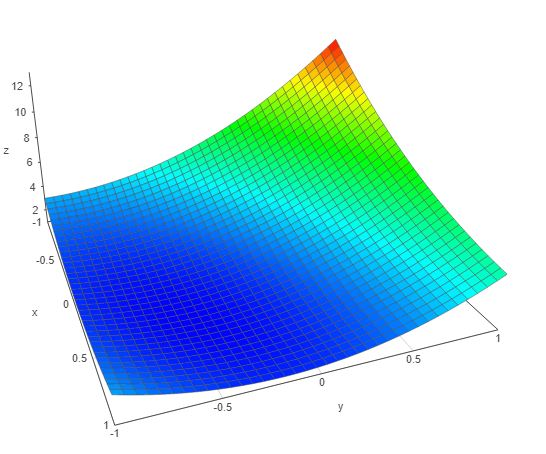
\includegraphics[scale=0.5]{plot134.jpg}\end{center}

Используя аналогичные рассуждения, для остальных планов можно получить:
\begin{enumerate}
	\item Для плана в точках $x^{(1)}, x^{(2)}, x^{(3)}$:
	$$d(x_1, x_2) \ge 2 + 3x_1 - x_2 -2x_1x_2 +\frac{5}{2}x_1^2 + \frac 3 2 x_2^2.$$
	Канонический вид поверхности:
	$$x^2 (4 - \sqrt{5}) + y^2 (4 + \sqrt 5) = 2z$$
	График поверхности:\\
	\begin{center}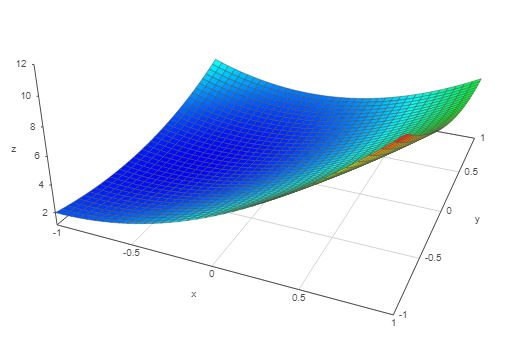
\includegraphics[scale=0.5]{plot123.jpg}\end{center}
	
	\item План в точках $x^{(1)}, x^{(2)}, x^{(4)}$:
	$$d(x_1, x_2) \ge 2 - 2x_1 - 2x_2 +3x_1x_2 +\frac{5}{2}x_1^2 + \frac 5 2 x_2^2$$
	Канонический вид поверхности:
	$$x^2 + 4y^2 = z$$
	График поверхности:\\
	\begin{center}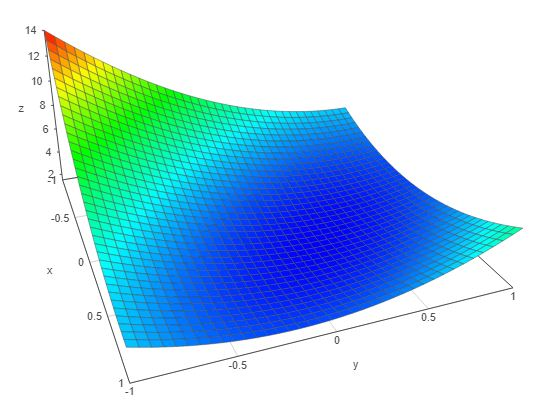
\includegraphics[scale=0.5]{plot124.jpg}\end{center}
	\item План в точках $x^{(2)}, x^{(3)}, x^{4)}$:
	$$d(x_1, x_2) \ge 2 + 2x_1 + 2x_2 +x_1x_2 +\frac{3}{2}x_1^2 + \frac 3 2 x_2^2$$
	Канонический вид поверхности:
	$$x^2 + 2 y^2 = z$$
	График поверхности:\\
	\begin{center}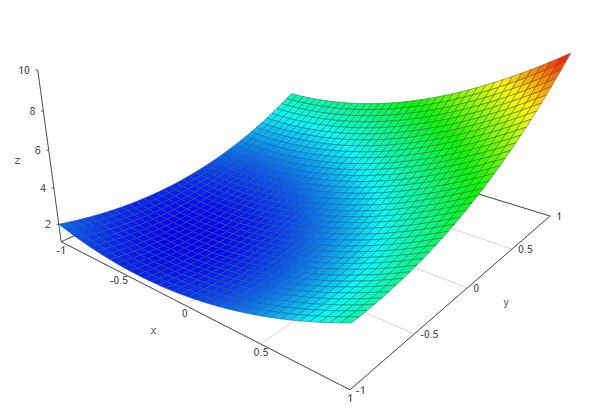
\includegraphics[scale=0.5]{plot234.jpg}\end{center}
\end{enumerate}

\subsection{Программная проверка оптимальности}
Подтвердим полученные результаты практически. Для этого была написана программа, которая перебирает все возможные планы исходной задачи и находит оптимальный.\\
Программа написана на языке Python с использованием пакетов numpy, scipy.\\
Приведем ее исходный код:
\lstinputlisting[language=Python,tabsize=2]{listings/check_optimal_in_points.py}

Вывод программы:
\lstinputlisting[numbers=none]{listings/check_optimal_in_points_output.txt}
Результат работы программы подтверждает теоретические рассуждения.


\subsection {Символьная проверка оптимальности}
В предыдущем параграфе оптимальность построенных планов была показана численно для заданной функции дисперсии. Покажем символьно, что неравенство \eqref{main-theorem:ineq} действительно обращается в равенство в вершинах спектра плана.\\
Для доказательства этого факта была написана программа в среде Matlab.
Указанная программа проверяет, что построенные планы в вершинах спектра плана в точности обращаются в значение дисперсии в заданной точке.
Приведём её листинг:
\lstinputlisting[language=Matlab,tabsize=2]{listings/symbol_check_optimality.txt}

Результат работы программы:
\lstinputlisting[numbers=none]{listings/symbol_check_optimality_output.txt}

Видно, что равенства выполняются.

\section{Точный D-оптимальный план для модели с линейным изменением}
\label{chapter2/diploma-section-2-2}
	
Рассмотрим следующую модель наблюдений:
\begin{equation} \label{linear-model:start}
y_i = \theta_0 + \theta_1 x_{i1} + \theta_2 x_{i2} + \varepsilon(x^{(i)}), |x_{i j}| \le 1, i = \overline{1, n}, j = \overline{1, 2}
\end{equation}
\begin{equation} \begin{split}
E\{\varepsilon(x^{(i)}) \varepsilon(x^{(j)}) \} = 0, i \ne j \\
E\{\varepsilon(x^{(i)}) = 0
\end{split}\end{equation}
\begin{equation}\label{linear-model:end}
D\{ \varepsilon( x^{(i)} ) \} = a_0 + a_1 x_{i1} + a_2 x_{i2},
a_0 > 0, |a_1| + |a_2| < a_0
\end{equation}
Справедлива следующая теорема.
\begin{theorem}
	Для модели наблюдений \eqref{linear-model:start}-\eqref{linear-model:end} существует точный $D$-оптимальный план, точки спектра которого лежат в вершинах единичного квадрата.
\end{theorem}
Доказательство данной теоремы может быть найдено в \cite{kirlitsa2017}.
Точный D-оптимальный план при заданном $n$ будет иметь следующий вид:
\begin{equation}
\varepsilon^{0} = \left \{ 
\underset{n_1} {x^{(1)}},
\underset{n_2} {x^{(2)}},
\underset{n_3} {x^{(3)}},
\underset{n_4} {x^{(4)}},
\right \}
\end{equation}
где $n_i$ - число наблюдений, которое нужно провести в точке $x^{(i)}$.\\
Однако числа $n_1, n_2, n_3, n_4$ не известны. Составим программу, которая для заданной функции дисперсии будет находить оптимальное размещение наблюдений в вершинах спектра плана.
Для этого воспользуемся тем фактом, что оптимальный план максимизирует определитель информационной матрицы Фишера $M(\varepsilon)$:
\begin{multline*} 
M(\varepsilon) = \sum_{i = 1}^{4} \frac{n_i} {d_i} 
\begin{pmatrix}1 \\ x_{i1} \\ x_{i2} \end{pmatrix}
(1, x_{i1}, x_{i2}) = \\
= \frac {n_1} {d_1} \begin{pmatrix}1 \\ 1 \\ 1\end{pmatrix} (1, 1, 1) + 
\frac {n_2} {d_2} \begin{pmatrix}1 \\ -1 \\ 1\end{pmatrix} (1, -1, 1) + \\
+ \frac {n_3} {d_3} \begin{pmatrix}1 \\ -1 \\ -1\end{pmatrix} (1, -1, -1) +
\frac {n_4)} {d_4} \begin{pmatrix} 1 \\ 1 \\ -1\end{pmatrix} (1, 1, -1) = \\
= \begin{pmatrix}
\lambda_1 + \lambda_2 + \lambda_3 + \lambda_4 &&
\lambda_1 - \lambda_2 - \lambda_3 + \lambda_4 &&
\lambda_1 + \lambda_2 - \lambda_3 - \lambda_4
\\
\lambda_1 - \lambda_2 - \lambda_3 + \lambda_4 &&
\lambda_1 + \lambda_2 + \lambda_3 + \lambda_4 &&
\lambda_1 - \lambda_2 + \lambda_3 - \lambda_4
\\
\lambda_1 + \lambda_2 - \lambda_3 - \lambda_4 &&
\lambda_1 - \lambda_2 + \lambda_3 - \lambda_4 &&
\lambda_1 + \lambda_2 + \lambda_3 + \lambda_4
\end{pmatrix} = \\
= \begin{pmatrix}
a && b && c \\
b && a && e \\
c && e && a
\end{pmatrix},
\end{multline*}
где
\begin{gather*}
\lambda_i = \frac {n_i} {d_i}, \\
a, b, c, e - \text{ соответствующие элемементы матрицы }.
\end{gather*}
Формулы для вычисления определителя подобной матрицы были получены нами ранее.

Тогда для нахождения оптимального плана необходимо перебрать различные наборы $n_1, n_2, n_3, n_4$ и посмотреть, какие из них максимизируют определитель информационной матрицы. Именно это и делает следующая программа на языке Python:

\lstinputlisting[language=Python]{listings/check_ns.py}

Вывод программы:
\lstinputlisting[numbers=none]{listings/check_ns_output.txt}


Для каждой поверхности $d(x_1, x_2)$ программа выводит массив оптимальных размещений наблюдений \textit{best placements}, каждый элемент которого есть $[n1, n2, n3, n4]$ -  количесто наблюдений в точках $x^{(1)}, x^{(2)}, x^{(3)}, x^{(4)}$ соответственно.\\
Проанализируем полученные результаты.\\
$n = 5$.\\
В первом случае рассматривается поверхность $d(x_1, x_2) \ge 40 + 0*x_1 + 0*x_2$, то есть равноточные наблюдения. В таких условиях существует 4 оптимальных плана, при которых в 3-х вершинах спектра по 1-му наблюдению и 2 наблюдения в 4-ой точке. \\
Далее рассматривается поверхность $d(x_1, x_2) \ge 40 - 1*x_1 + 0*x_2$. Видим, что при незначительном наклоне поверхности оптимальный план не изменяется. \\
Однако в случае $d(x_1, x_2) \ge 40 - 8*x_1 + 0*x_2$ существует уже только 2 оптимальных плана: 2 наблюдения размещаются в "менее поднятых" вершинах.\\
В критическом случае $d(x_1, x_2) \ge 40 - 39.5*x_1 + 0*x_2$ существует всего 1 оптимальный план.

\section{Точный D-оптимальный план для модели с тремя независимыми переменными}
\label{chapter2/diploma-section-2-3}
В пункте \ref{chapter2/diploma-section-2-1} была рассмотрена модель линейной регрессии \eqref{model:start}-\eqref{model:end} с тремя параметрами и двумя независимыми переменными.
Обобщим данную модель, вводя третью независимую переменную $x_0$:
\begin{gather} \label{model-3x:start}
y_i = \theta_0 x_{i0} + \theta_1 x_{i1} + \theta_2 x_{i2} + \varepsilon(x^{(i)}), i = \overline{1, n}, n \ge 3 \\
E\{ \varepsilon(x^{(i)}) \} = 0, E\{ \varepsilon^{(i)}\ \varepsilon^{(j)} \} = 0, i \ne j \\
D\{ \varepsilon(x^{(i)}) \} = d(x_{i0}, x_{i1}, x_{i2}) > 0, \\
d(x_0, x_1, x_2) \ge \frac{\sigma^2}{3}(x_0^2 + x_1^2 + x_2^2) \label{model-3x:end},
-1 \le x_{ij} \le 1, j = \overline{0, 2}, i = \overline{1, n},
\end{gather}
где $n$ -- число наблюдений, $x_{ij}$ -- независимые переменные, $x^{(i)} = (x_{i0}, x_{i1}, x_{i2})'$ -- вектор наблюдений, $\varepsilon(x^{(i)})$ -- случайные некоррелированные ошибки.

Таким образом все наблюдения находятся внутри куба c центром в точке $(0, 0, 0)$ и стороной 2.
Занумеруем вершины куба:
\begin{align*}
x^{(1)} = (1, 1, 1), && x^{(2)} = (1, -1, 1), && x^{(3)} = (1, -1, -1), && x^{(4)} = (1, 1, -1),\\
x^{(5)} = (-1, 1, 1), && x^{(6)} = (-1, -1, 1), && x^{(7)} = (-1, -1, -1), && x^{(8)} = (-1, 1, -1).
\end{align*}
Точки $x^{(1)}-x^{(4)}$ лежат на верхней грани куба и обозначены так же, как в модели \eqref{model:start}-\eqref{model:end}.\\
Также обозначим значение функции дисперсии в вершинах куба:
\begin{equation}
d_i = d(x^{(i)}), i = \overline{1, 8}.
\end{equation}

В теореме \ref{main-theorem} было показано, что для модели с двумя независимыми переменными \eqref{model:start}-\eqref{model:end} можно построить трёхточеный $D$-оптимальный план.  
Попробуем построить трёхточечный $D$-оптимальный план для модели с тремя независимыми переменными  \eqref{model-3x:start}-\eqref{model-3x:end}.
\begin{theorem}.\label{theorem:model-3x-D-opt}
	Для модели неравноточных наблюдений \eqref{model-3x:start}-\eqref{model-3x:end} следующие трехточечные планы являются непрерывными и $D$-оптимальными.\\
	План 
	\begin{equation} \label{theorem:model-3x-D-opt:plan-1}
	\varepsilon_1^{0} = \left \{ 
	\underset{\frac 1 3} {x^{(1)}},
	\underset{\frac 1 3} {x^{(2)}},
	\underset{\frac 1 3} {x^{(3)}}
	\right \},
	\end{equation}
	если для дисперсии наблюдений выполняется:
	\begin{multline}\label{theorem:model-3x-D-opt:plan-1-d}
	d(x_0, x_1, x_2) \ge \frac{d_{2} x_{1} x_{2}}{2} + x_{0}^{2} \left(\frac{d_{1}}{4} + \frac{d_{3}}{4}\right) + x_{0} \left(\frac{d_{1} x_{1}}{2} - \frac{d_{3} x_{2}}{2}\right) + \\ + x_{1}^{2} \left(\frac{d_{1}}{4} + \frac{d_{2}}{4}\right) + x_{2}^{2} \left(\frac{d_{2}}{4} + \frac{d_{3}}{4}\right).
	\end{multline}
	План 
	\begin{equation} \label{theorem:model-3x-D-opt:plan-2}
	\varepsilon_2^{0} = \left \{ 
	\underset{\frac 1 3} {x^{(1)}},
	\underset{\frac 1 3} {x^{(2)}},
	\underset{\frac 1 3} {x^{(4)}}
	\right \},
	\end{equation}
	если для дисперсии наблюдений выполняется:
	\begin{multline}\label{theorem:model-3x-D-opt:plan-2-d}
	d(x_0, x_1, x_2) \ge \frac{d_{1} x_{1} x_{2}}{2} + x_{0}^{2} \left(\frac{d_{2}}{4} + \frac{d_{4}}{4}\right) + x_{0} \left(- \frac{d_{2} x_{1}}{2} - \frac{d_{4} x_{2}}{2}\right) + \\ + x_{1}^{2} \left(\frac{d_{1}}{4} + \frac{d_{2}}{4}\right) + x_{2}^{2} \left(\frac{d_{1}}{4} + \frac{d_{4}}{4}\right).
	\end{multline}
	План 
	\begin{equation} \label{theorem:model-3x-D-opt:plan-3}
	\varepsilon_3^{0} = \left \{ 
	\underset{\frac 1 3} {x^{(1)}},
	\underset{\frac 1 3} {x^{(3)}},
	\underset{\frac 1 3} {x^{(4)}}
	\right \},
	\end{equation}
	если для дисперсии наблюдений выполняется:
	\begin{multline}\label{theorem:model-3x-D-opt:plan-3-d}
	d(x_0, x_1, x_2) \ge \frac{d_{4} x_{1} x_{2}}{2} + x_{0}^{2} \left(\frac{d_{1}}{4} + \frac{d_{3}}{4}\right) + x_{0} \left(\frac{d_{1} x_{2}}{2} - \frac{d_{3} x_{1}}{2}\right) + \\ + x_{1}^{2} \left(\frac{d_{3}}{4} + \frac{d_{4}}{4}\right) + x_{2}^{2} \left(\frac{d_{1}}{4} + \frac{d_{4}}{4}\right).
	\end{multline}
	План 
	\begin{equation} \label{theorem:model-3x-D-opt:plan-4}
	\varepsilon_4^{0} = \left \{ 
	\underset{\frac 1 3} {x^{(2)}},
	\underset{\frac 1 3} {x^{(3)}},
	\underset{\frac 1 3} {x^{(4)}}
	\right \},
	\end{equation}
	если для дисперсии наблюдений выполняется:
	\begin{multline}\label{theorem:model-3x-D-opt:plan-4-d}
	d(x_0, x_1, x_2) \ge \frac{d_{3} x_{1} x_{2}}{2} + x_{0}^{2} \left(\frac{d_{2}}{4} + \frac{d_{4}}{4}\right) + x_{0} \left(\frac{d_{2} x_{2}}{2} + \frac{d_{4} x_{1}}{2}\right) + \\ + x_{1}^{2} \left(\frac{d_{3}}{4} + \frac{d_{4}}{4}\right) + x_{2}^{2} \left(\frac{d_{2}}{4} + \frac{d_{3}}{4}\right).
	\end{multline}		
\end{theorem}

\textbf{Доказательство}. Доказательство данной теоремы производится аналогично доказательству теоремы \ref{main-theorem}. Для плана в точках $x^{(i)}, x^{(j)}, x^{(k)}$ запишем критерий эквавалентности Кифера-Вольфовица \eqref{theorem:model-3x-D-opt:KF-ineq}:
\begin{equation}\label{theorem:model-3x-D-opt:KF-ineq}
\frac{1}{d(x_0, x_1, x_2)} f'(x) M^{-1}(\varepsilon^0) f(x) \le 3,
\end{equation}
выразим $d(x_0, x_1, x_2)$ и покажем, что $d(x_0, x_1, x_2)$ равно заданным дисперсиям $d_i, d_j, d_k$ в соответствующих точках.

Ввиду объёмности и однотипности выкладок, описанная схема доказательства была реализована программно при помощи пакета компьютерной алгебры \textit{SymPy}  \cite{sympy}, написанном на языке программирования Python. Исходный код программы приведён в приложении \ref{appendix:3x_cube}.

Результат работы программы:
\lstinputlisting[numbers=none]{listings/3x_cube_output.txt}
Вывод показывает, что неравенства обращаются в равенства в точках спектра плана, что и требовалось доказать. \textbf{Теорема доказана}.\\

\textbf{Следствие}.
В теореме \ref{theorem:model-3x-D-opt} были рассмотрены планы, точки которых находятся на верхней грани куба. Куб имеет 6 граней, причём на каждой из них можно построить аналогичные планы. Данный факт следует из того, что точки планов на других гранях эквиваленты точкам одного из планов на верхней грани с точностью до переименования независимых переменных $x_0, x_1, x_2$ и домножения на $-1$. Таким образом доказано существование $24$-х планов для модели \eqref{model-3x:start}-\eqref{model-3x:end}.	



\section{Сравнение качества оценок точного D-оптимального и случайного планов на сгенерированных данных}
\label{chapter2/diploma-section-2-4}
В \ref{chapter2/diploma-section-2-1} и \ref{chapter2/diploma-section-2-2} была показана возможность построения точного $D$-оптимального плана для описанной модели наблюдений. Конечной целью эксперимента является оценка параметров модели по полученным наблюдениям. Далее исследуем: при каких условиях и на сколько оценки, полученные по наблюдениям в условиях $D$-оптимального плана, точнее оценок, полученных в результате наблюдений в случайных точках?

\subsection{Модель наблюдений}
Рассмотрим модель наблюдений из \ref{chapter2/diploma-section-2-1}.
Пусть было проведено $N$ наблюдений. Модель наблюдений имеет вид:
\begin{gather} \label{numerical-experiment:model:start}
y_i = \theta_0 + \theta_1 x_{i1} + \theta_2 x_{i2} + \varepsilon(x^{(i)}), i = \overline{1, N}, N \ge 3; \\
E\{ \varepsilon(x^{(i)}) \} = 0, E\{ \varepsilon^{(i)}\ \varepsilon^{(j)} \} = 0, i \ne j; \\
D\{ \varepsilon(x^{(i)}) \} = d(x_{i1}, x_{i2}) > 0; \\
d(x_1, x_2) \ge \frac{\sigma^2}{3}(1 + x_1^2 + x_2^2);
\label{numerical-experiment:model:end}
\end{gather}
где $\varepsilon^{(i)}$ - случайные, неравноточные и некоррелированные ошибки с дисперсией $d(x_{i1}, x_{i2})$. $-1 \le x_{ij} \le 1$, $i=\overline{1,N}, j=\overline{1, 2}$.\\
Введём обозначения для точек:
\begin{equation}\label{numerical-experiment:plan-points}
x^{(1)}=(1, 1), x^{(2)}=(-1, 1), x^{(3)}=(-1, -1), x^{(4)}=(1, -1).
\end{equation}
И для значений дисперсии наблюдений в этих точках:
\begin{equation}
d(x^{(1)}) = d_1, d(x^{(2)}) = d_2, d(x^{(3)}) = d_3, d(x^{(4)}) = d_4.
\end{equation}
Согласно теореме \ref{main-theorem}, для указанной модели план
\begin{equation} \label{numerical-expetiment:plan-1}
\varepsilon_1^{0} = \left \{ 
\underset{\frac 1 3} {x^{(1)}},
\underset{\frac 1 3} {x^{(2)}},
\underset{\frac 1 3} {x^{(3)}}
\right \}
\end{equation}
является точным $D$-оптимальным, если
\begin{equation}\label{numerical-experiment:d-eq}
d(x_1, x_2) \ge \frac 1 4 (d_1 + d_3 + 2 d_1 x_1 - 2 d_3 x_2 - 2d_2 x_1 x_2 + (d_1 + d_2)x_1^2 + (d_2 + d_3)x_2^2).
\end{equation}

Далее в этом разделе рассмотрим случай, когда неравенство \ref{numerical-experiment:d} обращается в равенство:
\begin{equation}\label{numerical-experiment:d}
d(x_1, x_2) = \frac 1 4 (d_1 + d_3 + 2 d_1 x_1 - 2 d_3 x_2 - 2d_2 x_1 x_2 + (d_1 + d_2)x_1^2 + (d_2 + d_3)x_2^2).
\end{equation}

\subsection {Взвешенный метод наименьших квадратов для оценки параметров}
Для оценки параметров регрессионной модели в условиях теоремы Гаусса-Маркова применяет метод наименьших квадратов (МНК). Неравноточность наблюдений нарушает условия теоремы Гаусса-Маркова, поэтому для оценки параметров неравноточной регрессионной модели применяется другой метод -- взвешенный метод наименьших квадратов (взвешенный МНК). Взвешенный МНК является обобщением МНК, при котором каждое наблюдение учитывается с весом, обратно пропорциональным его дисперсии. 

Обозначим $X$ - матрица плана эксперимента, $y = (y_1, ..., y_N)^T$ -- вектор наблюдений, $\varepsilon = (\varepsilon_1, ..., \varepsilon_N)^T$ -- вектор случайных ошибок, $\theta = (\theta_0, \theta_1, \theta_2)^T$ -- вектор параметров. Тогда \eqref{numerical-experiment:model:start} можно переписать в матричной форме:
\begin{equation}
y = X\theta + \varepsilon.
\end{equation}
Обозначим $w = (w_1, ..., w_N)^T$ -- вектор весов наблюдений, где $w_i = D(x_{i1}, x_{i2}) = d(x_{i1}, x_{i2})$. Также обозначим $W = diag(w)$ -- диагональная матрица весов.
Тогда $\hat \theta$ -- оценка вектора параметров $\theta$ по взвешенному МНК имеет вид:
\begin{equation}
\hat \theta = (X^T W X)^{-1} X^T W y.
\end{equation}

Обоснование и свойства взвешенного МНК могут быть найдены, например, в \cite{aivazian}.

\subsection{Численный эксперимент}
Проведём численный эксперимент, чтобы понять, при каких условиях и на сколько $D$-оптимальный план эффективнее другого, случайного плана.
\subsubsection{Алгоритм проведения эксперимента.}
\begin{enumerate}
	\item \label{numerical-experiment:algo:loop:start}задать коэффициенты $\theta_0, \theta_1, \theta_2$ уравнения регрессии \eqref{numerical-experiment:model:start}, значения $d_1, d_2, d_3$ и, соответственно, функцию $d(x_1, x_2)$ согласно \eqref{numerical-experiment:d};
	\item задать количество наблюдений $N$, где $N$ кратно 3;
	\item сгенерировать матрицу плана эксперимента $X$ одним из способов:
		\begin{enumerate}
			\item $X = X_{optimal}$ -- согласно теореме о $D$-оптимальном плане, т.е. $N/3$ наблюдений в каждой из точек $x^{(1)}, x^{(2)}, x^{(3)}$;
			\item $X = X_{random}$ -- $N$ случайных точек из двумерного равномерного распределения $R^2[-1, 1]$;
		\end{enumerate}
	\item для $X$ сгенерировать вектор ошибок $\varepsilon$ с дисперсией $d(x_1, x_2)$;
	\item вычислить $y = X \theta + \varepsilon$;
	\item по взвешенному методу наименьших квадратов найти  $\hat \theta$ -- оценку вектора параметров $\theta$;
	\item \label{numerical-experiment:algo:loop:end} измерить точность оценки как среднеквадратическую ошибку: $e = \frac 1 3 \sum_{i=0}^{2} (\theta_i - \hat \theta_i)^2$. 
\end{enumerate}

Чтобы сделать результаты эксперимента более точными, описанный алгоритм повторяется $T$ раз и в качестве итоговой оценки точности берётся $\overline e = \frac 1 T \sum_{t=1}^{T} e_t$.

\subsubsection{Параметры эксперимента.}
Зададим конкретные значения параметров для проведения эксперимента.
\begin{enumerate}
	\item $\theta = (2, 5, 1)^T$;
	\item $d_1 = 6, d_2 = 4, d_3 = 2$;
	\item $N \in \{3, 6, ..., 24, 27\}$;
	\item $T = 5$.
\end{enumerate} 

\subsubsection{Реализация эксперимента.}
Для реализация описанного эксперимента была написана программа на языке программирования \textit{Python} с использованием пакетов \textit{NumPy}, \textit{SciPy}, \textit{scikit-learn}.
Её исходных код приведён ниже.
\lstinputlisting[language=Python,tabsize=2]{listings/heteroscedastic_experiment.py}

\subsubsection{Результаты эксперимента.}
Рассмотрим график изменения средней квадратичной ошибки оценок в зависимости от числа проведённых наблюдений. Закрашенная область соответствует $\overline e$ с учётом стандартного отклонения $\overline r$. Синяя линяя соответствует оптимальному плану, оранжевая - случайному.
\begin{center}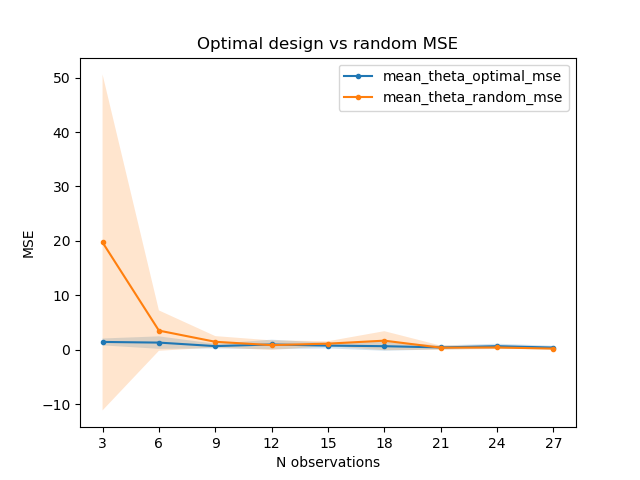
\includegraphics[scale=1.0]{heteroscedastic-experiment.png}\end{center} 

Видно, что $D$-оптимальный план эксперимента позволяет точно оценить параметры модели уже при $N=3$, в то время как случайный план является крайне неточными при $N < 9$. При $N > 9$ оба подхода дают почти одинаково точный результат.

Таким образом $D$-оптимальный план позволяет существенно снизить число проводимых наблюдений при достижении той же точности оценок.





%%% описание главы 3

% \stepcounter{chapter}
% \phantomsection
% \chapter*{ГЛАВА 3\\
%  НАЗВАНИЕ ГЛАВЫ}
% \addcontentsline{toc}{chapter}{Глава 3. Название главы}
% \setcounter{section}{0}

% \section{Название раздела}

\subsection{Название подраздела}

\subsubsection{Название пункта}

Lorem ipsum dolor sit amet, consectetur adipiscing elit. Fusce ultrices finibus arcu in tincidunt.
Curabitur pellentesque purus vel aliquet efficitur. Morbi quis placerat diam. Curabitur id fringilla
nibh, eu volutpat tellus. Sed nec fermentum magna, eget blandit ipsum. Aenean fermentum ipsum eu
luctus vulputate. In hendrerit eros nibh, non pretium eros malesuada nec. Donec enim lectus, convallis
id scelerisque a, molestie nec neque.

Integer fermentum, dui volutpat suscipit scelerisque, orci sapien suscipit mauris, nec bibendum est
enim elementum sem. Mauris pharetra turpis eget ex tincidunt, in efficitur mi dictum. Suspendisse
convallis non lacus nec fermentum. Suspendisse eleifend enim odio, sed eleifend felis luctus eget.
In bibendum nulla a lorem tempor dignissim. Nunc tempor arcu a nisl feugiat, a fermentum ante eleifend.
Etiam sed augue lacinia, luctus odio sed, dapibus lacus. Pellentesque suscipit mauris vitae est
fringilla consequat. Sed dui est, varius sit amet auctor ut, euismod a magna. Vivamus tristique leo
ligula, non lacinia justo volutpat in. Maecenas eu mi velit. Sed vel elit ligula. In imperdiet varius
elit, at rutrum mauris lobortis nec. Suspendisse quis orci id urna porta eleifend.

Curabitur pellentesque nunc ut urna elementum bibendum. Maecenas sit amet ante tincidunt, dictum
neque et, eleifend felis. Pellentesque rhoncus mi ut mauris ullamcorper pretium. Maecenas non blandit
ex, quis elementum leo. Donec ultricies, velit in ultricies fringilla, turpis neque facilisis eros,
non congue ipsum sapien id enim. Praesent vitae tellus ornare orci mattis ornare et ut sapien. Quisque
iaculis lorem mauris. Phasellus eu arcu placerat, convallis velit at, tincidunt velit. Nulla eget
vestibulum erat. Fusce eu ipsum rutrum, varius felis dictum, aliquam augue.

In dignissim odio eget porttitor malesuada. Pellentesque venenatis urna eget risus facilisis
imperdiet. Donec ligula neque, volutpat ut leo in, interdum pellentesque metus. Nam mattis ligula
nec volutpat fringilla. Pellentesque nec semper mauris, non condimentum metus. Ut imperdiet sapien
nec pretium porta. Nam id arcu non nibh ultricies consectetur id sed dui.

Duis semper luctus posuere. Donec aliquet quam a ex posuere venenatis. Aliquam interdum suscipit
justo, placerat auctor lacus feugiat eget. Aliquam vulputate vitae lorem at molestie. In iaculis
felis in felis rutrum, eget finibus nunc gravida. Curabitur tortor tortor, rutrum eu urna ut, commodo
tempor justo. Quisque at tortor nec leo fringilla posuere.

Fusce sapien nisl, gravida et eleifend vitae, finibus at quam. Curabitur quis venenatis nisl.
Aenean in rhoncus magna. In hac habitasse platea dictumst. Nulla id feugiat nibh. Suspendisse ut
ligula at elit auctor aliquet. Quisque dolor nunc, pretium vitae posuere dapibus, molestie ac lectus.
Nulla tempor dui lacinia auctor finibus. Curabitur placerat diam non augue posuere accumsan. Nunc
laoreet urna mi, eget faucibus ligula faucibus at. Nunc eu laoreet erat. Suspendisse varius est orci,
ut scelerisque metus faucibus non. Donec luctus et massa non semper. Nullam non augue enim. Aliquam
vitae convallis ligula. Interdum et malesuada fames ac ante ipsum primis in faucibus.

\begin{figure}
  
\includegraphics[width=\linewidth]{pics/hardcore.jpg}
  \caption{Учеба - это хардкор. Диплом - это дважды хардкор.}
  %\label{fig:hard}
\end{figure}


\subsubsection{Название пункта}

Lorem ipsum dolor sit amet, consectetur adipiscing elit. Fusce ultrices finibus arcu in tincidunt.
Curabitur pellentesque purus vel aliquet efficitur. Morbi quis placerat diam. Curabitur id fringilla
nibh, eu volutpat tellus. Sed nec fermentum magna, eget blandit ipsum. Aenean fermentum ipsum eu
luctus vulputate. In hendrerit eros nibh, non pretium eros malesuada nec. Donec enim lectus, convallis
id scelerisque a, molestie nec neque.

Integer fermentum, dui volutpat suscipit scelerisque, orci sapien suscipit mauris, nec bibendum est
enim elementum sem. Mauris pharetra turpis eget ex tincidunt, in efficitur mi dictum. Suspendisse
convallis non lacus nec fermentum. Suspendisse eleifend enim odio, sed eleifend felis luctus eget.
In bibendum nulla a lorem tempor dignissim. Nunc tempor arcu a nisl feugiat, a fermentum ante eleifend.
Etiam sed augue lacinia, luctus odio sed, dapibus lacus. Pellentesque suscipit mauris vitae est
fringilla consequat. Sed dui est, varius sit amet auctor ut, euismod a magna. Vivamus tristique leo
ligula, non lacinia justo volutpat in. Maecenas eu mi velit. Sed vel elit ligula. In imperdiet varius
elit, at rutrum mauris lobortis nec. Suspendisse quis orci id urna porta eleifend.

Curabitur pellentesque nunc ut urna elementum bibendum. Maecenas sit amet ante tincidunt, dictum
neque et, eleifend felis. Pellentesque rhoncus mi ut mauris ullamcorper pretium. Maecenas non blandit
ex, quis elementum leo. Donec ultricies, velit in ultricies fringilla, turpis neque facilisis eros,
non congue ipsum sapien id enim. Praesent vitae tellus ornare orci mattis ornare et ut sapien. Quisque
iaculis lorem mauris. Phasellus eu arcu placerat, convallis velit at, tincidunt velit. Nulla eget
vestibulum erat. Fusce eu ipsum rutrum, varius felis dictum, aliquam augue.

In dignissim odio eget porttitor malesuada. Pellentesque venenatis urna eget risus facilisis
imperdiet. Donec ligula neque, volutpat ut leo in, interdum pellentesque metus. Nam mattis ligula
nec volutpat fringilla. Pellentesque nec semper mauris, non condimentum metus. Ut imperdiet sapien
nec pretium porta. Nam id arcu non nibh ultricies consectetur id sed dui.

Duis semper luctus posuere. Donec aliquet quam a ex posuere venenatis. Aliquam interdum suscipit
justo, placerat auctor lacus feugiat eget. Aliquam vulputate vitae lorem at molestie. In iaculis
felis in felis rutrum, eget finibus nunc gravida. Curabitur tortor tortor, rutrum eu urna ut, commodo
tempor justo. Quisque at tortor nec leo fringilla posuere.

Fusce sapien nisl, gravida et eleifend vitae, finibus at quam. Curabitur quis venenatis nisl.
Aenean in rhoncus magna. In hac habitasse platea dictumst. Nulla id feugiat nibh. Suspendisse ut
ligula at elit auctor aliquet. Quisque dolor nunc, pretium vitae posuere dapibus, molestie ac lectus.
Nulla tempor dui lacinia auctor finibus. Curabitur placerat diam non augue posuere accumsan. Nunc
laoreet urna mi, eget faucibus ligula faucibus at. Nunc eu laoreet erat. Suspendisse varius est orci,
ut scelerisque metus faucibus non. Donec luctus et massa non semper. Nullam non augue enim. Aliquam
vitae convallis ligula. Interdum et malesuada fames ac ante ipsum primis in faucibus.

\begin{figure}
  
\includegraphics[width=\linewidth]{pics/hardcore.jpg}
  \caption{Учеба - это хардкор. Диплом - это дважды хардкор.}
  %\label{fig:hard}
\end{figure}


\subsubsection{Название пункта}

Lorem ipsum dolor sit amet, consectetur adipiscing elit. Fusce ultrices finibus arcu in tincidunt.
Curabitur pellentesque purus vel aliquet efficitur. Morbi quis placerat diam. Curabitur id fringilla
nibh, eu volutpat tellus. Sed nec fermentum magna, eget blandit ipsum. Aenean fermentum ipsum eu
luctus vulputate. In hendrerit eros nibh, non pretium eros malesuada nec. Donec enim lectus, convallis
id scelerisque a, molestie nec neque.

Integer fermentum, dui volutpat suscipit scelerisque, orci sapien suscipit mauris, nec bibendum est
enim elementum sem. Mauris pharetra turpis eget ex tincidunt, in efficitur mi dictum. Suspendisse
convallis non lacus nec fermentum. Suspendisse eleifend enim odio, sed eleifend felis luctus eget.
In bibendum nulla a lorem tempor dignissim. Nunc tempor arcu a nisl feugiat, a fermentum ante eleifend.
Etiam sed augue lacinia, luctus odio sed, dapibus lacus. Pellentesque suscipit mauris vitae est
fringilla consequat. Sed dui est, varius sit amet auctor ut, euismod a magna. Vivamus tristique leo
ligula, non lacinia justo volutpat in. Maecenas eu mi velit. Sed vel elit ligula. In imperdiet varius
elit, at rutrum mauris lobortis nec. Suspendisse quis orci id urna porta eleifend.

Curabitur pellentesque nunc ut urna elementum bibendum. Maecenas sit amet ante tincidunt, dictum
neque et, eleifend felis. Pellentesque rhoncus mi ut mauris ullamcorper pretium. Maecenas non blandit
ex, quis elementum leo. Donec ultricies, velit in ultricies fringilla, turpis neque facilisis eros,
non congue ipsum sapien id enim. Praesent vitae tellus ornare orci mattis ornare et ut sapien. Quisque
iaculis lorem mauris. Phasellus eu arcu placerat, convallis velit at, tincidunt velit. Nulla eget
vestibulum erat. Fusce eu ipsum rutrum, varius felis dictum, aliquam augue.

In dignissim odio eget porttitor malesuada. Pellentesque venenatis urna eget risus facilisis
imperdiet. Donec ligula neque, volutpat ut leo in, interdum pellentesque metus. Nam mattis ligula
nec volutpat fringilla. Pellentesque nec semper mauris, non condimentum metus. Ut imperdiet sapien
nec pretium porta. Nam id arcu non nibh ultricies consectetur id sed dui.

Duis semper luctus posuere. Donec aliquet quam a ex posuere venenatis. Aliquam interdum suscipit
justo, placerat auctor lacus feugiat eget. Aliquam vulputate vitae lorem at molestie. In iaculis
felis in felis rutrum, eget finibus nunc gravida. Curabitur tortor tortor, rutrum eu urna ut, commodo
tempor justo. Quisque at tortor nec leo fringilla posuere.

Fusce sapien nisl, gravida et eleifend vitae, finibus at quam. Curabitur quis venenatis nisl.
Aenean in rhoncus magna. In hac habitasse platea dictumst. Nulla id feugiat nibh. Suspendisse ut
ligula at elit auctor aliquet. Quisque dolor nunc, pretium vitae posuere dapibus, molestie ac lectus.
Nulla tempor dui lacinia auctor finibus. Curabitur placerat diam non augue posuere accumsan. Nunc
laoreet urna mi, eget faucibus ligula faucibus at. Nunc eu laoreet erat. Suspendisse varius est orci,
ut scelerisque metus faucibus non. Donec luctus et massa non semper. Nullam non augue enim. Aliquam
vitae convallis ligula. Interdum et malesuada fames ac ante ipsum primis in faucibus.

\begin{figure}
  
\includegraphics[width=\linewidth]{pics/hardcore.jpg}
  \caption{Учеба - это хардкор. Диплом - это дважды хардкор.}
  %\label{fig:hard}
\end{figure}


\subsection{Название подраздела}

\subsubsection{Название пункта}

Lorem ipsum dolor sit amet, consectetur adipiscing elit. Fusce ultrices finibus arcu in tincidunt.
Curabitur pellentesque purus vel aliquet efficitur. Morbi quis placerat diam. Curabitur id fringilla
nibh, eu volutpat tellus. Sed nec fermentum magna, eget blandit ipsum. Aenean fermentum ipsum eu
luctus vulputate. In hendrerit eros nibh, non pretium eros malesuada nec. Donec enim lectus, convallis
id scelerisque a, molestie nec neque.

Integer fermentum, dui volutpat suscipit scelerisque, orci sapien suscipit mauris, nec bibendum est
enim elementum sem. Mauris pharetra turpis eget ex tincidunt, in efficitur mi dictum. Suspendisse
convallis non lacus nec fermentum. Suspendisse eleifend enim odio, sed eleifend felis luctus eget.
In bibendum nulla a lorem tempor dignissim. Nunc tempor arcu a nisl feugiat, a fermentum ante eleifend.
Etiam sed augue lacinia, luctus odio sed, dapibus lacus. Pellentesque suscipit mauris vitae est
fringilla consequat. Sed dui est, varius sit amet auctor ut, euismod a magna. Vivamus tristique leo
ligula, non lacinia justo volutpat in. Maecenas eu mi velit. Sed vel elit ligula. In imperdiet varius
elit, at rutrum mauris lobortis nec. Suspendisse quis orci id urna porta eleifend.

Curabitur pellentesque nunc ut urna elementum bibendum. Maecenas sit amet ante tincidunt, dictum
neque et, eleifend felis. Pellentesque rhoncus mi ut mauris ullamcorper pretium. Maecenas non blandit
ex, quis elementum leo. Donec ultricies, velit in ultricies fringilla, turpis neque facilisis eros,
non congue ipsum sapien id enim. Praesent vitae tellus ornare orci mattis ornare et ut sapien. Quisque
iaculis lorem mauris. Phasellus eu arcu placerat, convallis velit at, tincidunt velit. Nulla eget
vestibulum erat. Fusce eu ipsum rutrum, varius felis dictum, aliquam augue.

In dignissim odio eget porttitor malesuada. Pellentesque venenatis urna eget risus facilisis
imperdiet. Donec ligula neque, volutpat ut leo in, interdum pellentesque metus. Nam mattis ligula
nec volutpat fringilla. Pellentesque nec semper mauris, non condimentum metus. Ut imperdiet sapien
nec pretium porta. Nam id arcu non nibh ultricies consectetur id sed dui.

Duis semper luctus posuere. Donec aliquet quam a ex posuere venenatis. Aliquam interdum suscipit
justo, placerat auctor lacus feugiat eget. Aliquam vulputate vitae lorem at molestie. In iaculis
felis in felis rutrum, eget finibus nunc gravida. Curabitur tortor tortor, rutrum eu urna ut, commodo
tempor justo. Quisque at tortor nec leo fringilla posuere.

Fusce sapien nisl, gravida et eleifend vitae, finibus at quam. Curabitur quis venenatis nisl.
Aenean in rhoncus magna. In hac habitasse platea dictumst. Nulla id feugiat nibh. Suspendisse ut
ligula at elit auctor aliquet. Quisque dolor nunc, pretium vitae posuere dapibus, molestie ac lectus.
Nulla tempor dui lacinia auctor finibus. Curabitur placerat diam non augue posuere accumsan. Nunc
laoreet urna mi, eget faucibus ligula faucibus at. Nunc eu laoreet erat. Suspendisse varius est orci,
ut scelerisque metus faucibus non. Donec luctus et massa non semper. Nullam non augue enim. Aliquam
vitae convallis ligula. Interdum et malesuada fames ac ante ipsum primis in faucibus.

\begin{figure}
  
\includegraphics[width=\linewidth]{pics/hardcore.jpg}
  \caption{Учеба - это хардкор. Диплом - это дважды хардкор.}
  %\label{fig:hard}
\end{figure}


\subsubsection{Название пункта}

Lorem ipsum dolor sit amet, consectetur adipiscing elit. Fusce ultrices finibus arcu in tincidunt.
Curabitur pellentesque purus vel aliquet efficitur. Morbi quis placerat diam. Curabitur id fringilla
nibh, eu volutpat tellus. Sed nec fermentum magna, eget blandit ipsum. Aenean fermentum ipsum eu
luctus vulputate. In hendrerit eros nibh, non pretium eros malesuada nec. Donec enim lectus, convallis
id scelerisque a, molestie nec neque.

Integer fermentum, dui volutpat suscipit scelerisque, orci sapien suscipit mauris, nec bibendum est
enim elementum sem. Mauris pharetra turpis eget ex tincidunt, in efficitur mi dictum. Suspendisse
convallis non lacus nec fermentum. Suspendisse eleifend enim odio, sed eleifend felis luctus eget.
In bibendum nulla a lorem tempor dignissim. Nunc tempor arcu a nisl feugiat, a fermentum ante eleifend.
Etiam sed augue lacinia, luctus odio sed, dapibus lacus. Pellentesque suscipit mauris vitae est
fringilla consequat. Sed dui est, varius sit amet auctor ut, euismod a magna. Vivamus tristique leo
ligula, non lacinia justo volutpat in. Maecenas eu mi velit. Sed vel elit ligula. In imperdiet varius
elit, at rutrum mauris lobortis nec. Suspendisse quis orci id urna porta eleifend.

Curabitur pellentesque nunc ut urna elementum bibendum. Maecenas sit amet ante tincidunt, dictum
neque et, eleifend felis. Pellentesque rhoncus mi ut mauris ullamcorper pretium. Maecenas non blandit
ex, quis elementum leo. Donec ultricies, velit in ultricies fringilla, turpis neque facilisis eros,
non congue ipsum sapien id enim. Praesent vitae tellus ornare orci mattis ornare et ut sapien. Quisque
iaculis lorem mauris. Phasellus eu arcu placerat, convallis velit at, tincidunt velit. Nulla eget
vestibulum erat. Fusce eu ipsum rutrum, varius felis dictum, aliquam augue.

In dignissim odio eget porttitor malesuada. Pellentesque venenatis urna eget risus facilisis
imperdiet. Donec ligula neque, volutpat ut leo in, interdum pellentesque metus. Nam mattis ligula
nec volutpat fringilla. Pellentesque nec semper mauris, non condimentum metus. Ut imperdiet sapien
nec pretium porta. Nam id arcu non nibh ultricies consectetur id sed dui.

Duis semper luctus posuere. Donec aliquet quam a ex posuere venenatis. Aliquam interdum suscipit
justo, placerat auctor lacus feugiat eget. Aliquam vulputate vitae lorem at molestie. In iaculis
felis in felis rutrum, eget finibus nunc gravida. Curabitur tortor tortor, rutrum eu urna ut, commodo
tempor justo. Quisque at tortor nec leo fringilla posuere.

Fusce sapien nisl, gravida et eleifend vitae, finibus at quam. Curabitur quis venenatis nisl.
Aenean in rhoncus magna. In hac habitasse platea dictumst. Nulla id feugiat nibh. Suspendisse ut
ligula at elit auctor aliquet. Quisque dolor nunc, pretium vitae posuere dapibus, molestie ac lectus.
Nulla tempor dui lacinia auctor finibus. Curabitur placerat diam non augue posuere accumsan. Nunc
laoreet urna mi, eget faucibus ligula faucibus at. Nunc eu laoreet erat. Suspendisse varius est orci,
ut scelerisque metus faucibus non. Donec luctus et massa non semper. Nullam non augue enim. Aliquam
vitae convallis ligula. Interdum et malesuada fames ac ante ipsum primis in faucibus.

\begin{figure}
  
\includegraphics[width=\linewidth]{pics/hardcore.jpg}
  \caption{Учеба - это хардкор. Диплом - это дважды хардкор.}
  %\label{fig:hard}
\end{figure}



\section{Название раздела}

\subsection{Название подраздела}

\subsubsection{Название пункта}

Lorem ipsum dolor sit amet, consectetur adipiscing elit. Fusce ultrices finibus arcu in tincidunt.
Curabitur pellentesque purus vel aliquet efficitur. Morbi quis placerat diam. Curabitur id fringilla
nibh, eu volutpat tellus. Sed nec fermentum magna, eget blandit ipsum. Aenean fermentum ipsum eu
luctus vulputate. In hendrerit eros nibh, non pretium eros malesuada nec. Donec enim lectus, convallis
id scelerisque a, molestie nec neque.

Integer fermentum, dui volutpat suscipit scelerisque, orci sapien suscipit mauris, nec bibendum est
enim elementum sem. Mauris pharetra turpis eget ex tincidunt, in efficitur mi dictum. Suspendisse
convallis non lacus nec fermentum. Suspendisse eleifend enim odio, sed eleifend felis luctus eget.
In bibendum nulla a lorem tempor dignissim. Nunc tempor arcu a nisl feugiat, a fermentum ante eleifend.
Etiam sed augue lacinia, luctus odio sed, dapibus lacus. Pellentesque suscipit mauris vitae est
fringilla consequat. Sed dui est, varius sit amet auctor ut, euismod a magna. Vivamus tristique leo
ligula, non lacinia justo volutpat in. Maecenas eu mi velit. Sed vel elit ligula. In imperdiet varius
elit, at rutrum mauris lobortis nec. Suspendisse quis orci id urna porta eleifend.

Curabitur pellentesque nunc ut urna elementum bibendum. Maecenas sit amet ante tincidunt, dictum
neque et, eleifend felis. Pellentesque rhoncus mi ut mauris ullamcorper pretium. Maecenas non blandit
ex, quis elementum leo. Donec ultricies, velit in ultricies fringilla, turpis neque facilisis eros,
non congue ipsum sapien id enim. Praesent vitae tellus ornare orci mattis ornare et ut sapien. Quisque
iaculis lorem mauris. Phasellus eu arcu placerat, convallis velit at, tincidunt velit. Nulla eget
vestibulum erat. Fusce eu ipsum rutrum, varius felis dictum, aliquam augue.

In dignissim odio eget porttitor malesuada. Pellentesque venenatis urna eget risus facilisis
imperdiet. Donec ligula neque, volutpat ut leo in, interdum pellentesque metus. Nam mattis ligula
nec volutpat fringilla. Pellentesque nec semper mauris, non condimentum metus. Ut imperdiet sapien
nec pretium porta. Nam id arcu non nibh ultricies consectetur id sed dui.

Duis semper luctus posuere. Donec aliquet quam a ex posuere venenatis. Aliquam interdum suscipit
justo, placerat auctor lacus feugiat eget. Aliquam vulputate vitae lorem at molestie. In iaculis
felis in felis rutrum, eget finibus nunc gravida. Curabitur tortor tortor, rutrum eu urna ut, commodo
tempor justo. Quisque at tortor nec leo fringilla posuere.

Fusce sapien nisl, gravida et eleifend vitae, finibus at quam. Curabitur quis venenatis nisl.
Aenean in rhoncus magna. In hac habitasse platea dictumst. Nulla id feugiat nibh. Suspendisse ut
ligula at elit auctor aliquet. Quisque dolor nunc, pretium vitae posuere dapibus, molestie ac lectus.
Nulla tempor dui lacinia auctor finibus. Curabitur placerat diam non augue posuere accumsan. Nunc
laoreet urna mi, eget faucibus ligula faucibus at. Nunc eu laoreet erat. Suspendisse varius est orci,
ut scelerisque metus faucibus non. Donec luctus et massa non semper. Nullam non augue enim. Aliquam
vitae convallis ligula. Interdum et malesuada fames ac ante ipsum primis in faucibus.

\begin{figure}
  
\includegraphics[width=\linewidth]{pics/hardcore.jpg}
  \caption{Учеба - это хардкор. Диплом - это дважды хардкор.}
  %\label{fig:hard}
\end{figure}


\subsubsection{Название пункта}

Lorem ipsum dolor sit amet, consectetur adipiscing elit. Fusce ultrices finibus arcu in tincidunt.
Curabitur pellentesque purus vel aliquet efficitur. Morbi quis placerat diam. Curabitur id fringilla
nibh, eu volutpat tellus. Sed nec fermentum magna, eget blandit ipsum. Aenean fermentum ipsum eu
luctus vulputate. In hendrerit eros nibh, non pretium eros malesuada nec. Donec enim lectus, convallis
id scelerisque a, molestie nec neque.

Integer fermentum, dui volutpat suscipit scelerisque, orci sapien suscipit mauris, nec bibendum est
enim elementum sem. Mauris pharetra turpis eget ex tincidunt, in efficitur mi dictum. Suspendisse
convallis non lacus nec fermentum. Suspendisse eleifend enim odio, sed eleifend felis luctus eget.
In bibendum nulla a lorem tempor dignissim. Nunc tempor arcu a nisl feugiat, a fermentum ante eleifend.
Etiam sed augue lacinia, luctus odio sed, dapibus lacus. Pellentesque suscipit mauris vitae est
fringilla consequat. Sed dui est, varius sit amet auctor ut, euismod a magna. Vivamus tristique leo
ligula, non lacinia justo volutpat in. Maecenas eu mi velit. Sed vel elit ligula. In imperdiet varius
elit, at rutrum mauris lobortis nec. Suspendisse quis orci id urna porta eleifend.

Curabitur pellentesque nunc ut urna elementum bibendum. Maecenas sit amet ante tincidunt, dictum
neque et, eleifend felis. Pellentesque rhoncus mi ut mauris ullamcorper pretium. Maecenas non blandit
ex, quis elementum leo. Donec ultricies, velit in ultricies fringilla, turpis neque facilisis eros,
non congue ipsum sapien id enim. Praesent vitae tellus ornare orci mattis ornare et ut sapien. Quisque
iaculis lorem mauris. Phasellus eu arcu placerat, convallis velit at, tincidunt velit. Nulla eget
vestibulum erat. Fusce eu ipsum rutrum, varius felis dictum, aliquam augue.

In dignissim odio eget porttitor malesuada. Pellentesque venenatis urna eget risus facilisis
imperdiet. Donec ligula neque, volutpat ut leo in, interdum pellentesque metus. Nam mattis ligula
nec volutpat fringilla. Pellentesque nec semper mauris, non condimentum metus. Ut imperdiet sapien
nec pretium porta. Nam id arcu non nibh ultricies consectetur id sed dui.

Duis semper luctus posuere. Donec aliquet quam a ex posuere venenatis. Aliquam interdum suscipit
justo, placerat auctor lacus feugiat eget. Aliquam vulputate vitae lorem at molestie. In iaculis
felis in felis rutrum, eget finibus nunc gravida. Curabitur tortor tortor, rutrum eu urna ut, commodo
tempor justo. Quisque at tortor nec leo fringilla posuere.

Fusce sapien nisl, gravida et eleifend vitae, finibus at quam. Curabitur quis venenatis nisl.
Aenean in rhoncus magna. In hac habitasse platea dictumst. Nulla id feugiat nibh. Suspendisse ut
ligula at elit auctor aliquet. Quisque dolor nunc, pretium vitae posuere dapibus, molestie ac lectus.
Nulla tempor dui lacinia auctor finibus. Curabitur placerat diam non augue posuere accumsan. Nunc
laoreet urna mi, eget faucibus ligula faucibus at. Nunc eu laoreet erat. Suspendisse varius est orci,
ut scelerisque metus faucibus non. Donec luctus et massa non semper. Nullam non augue enim. Aliquam
vitae convallis ligula. Interdum et malesuada fames ac ante ipsum primis in faucibus.

\begin{figure}
  
\includegraphics[width=\linewidth]{pics/hardcore.jpg}
  \caption{Учеба - это хардкор. Диплом - это дважды хардкор.}
  %\label{fig:hard}
\end{figure}


\subsubsection{Название пункта}

Lorem ipsum dolor sit amet, consectetur adipiscing elit. Fusce ultrices finibus arcu in tincidunt.
Curabitur pellentesque purus vel aliquet efficitur. Morbi quis placerat diam. Curabitur id fringilla
nibh, eu volutpat tellus. Sed nec fermentum magna, eget blandit ipsum. Aenean fermentum ipsum eu
luctus vulputate. In hendrerit eros nibh, non pretium eros malesuada nec. Donec enim lectus, convallis
id scelerisque a, molestie nec neque.

Integer fermentum, dui volutpat suscipit scelerisque, orci sapien suscipit mauris, nec bibendum est
enim elementum sem. Mauris pharetra turpis eget ex tincidunt, in efficitur mi dictum. Suspendisse
convallis non lacus nec fermentum. Suspendisse eleifend enim odio, sed eleifend felis luctus eget.
In bibendum nulla a lorem tempor dignissim. Nunc tempor arcu a nisl feugiat, a fermentum ante eleifend.
Etiam sed augue lacinia, luctus odio sed, dapibus lacus. Pellentesque suscipit mauris vitae est
fringilla consequat. Sed dui est, varius sit amet auctor ut, euismod a magna. Vivamus tristique leo
ligula, non lacinia justo volutpat in. Maecenas eu mi velit. Sed vel elit ligula. In imperdiet varius
elit, at rutrum mauris lobortis nec. Suspendisse quis orci id urna porta eleifend.

Curabitur pellentesque nunc ut urna elementum bibendum. Maecenas sit amet ante tincidunt, dictum
neque et, eleifend felis. Pellentesque rhoncus mi ut mauris ullamcorper pretium. Maecenas non blandit
ex, quis elementum leo. Donec ultricies, velit in ultricies fringilla, turpis neque facilisis eros,
non congue ipsum sapien id enim. Praesent vitae tellus ornare orci mattis ornare et ut sapien. Quisque
iaculis lorem mauris. Phasellus eu arcu placerat, convallis velit at, tincidunt velit. Nulla eget
vestibulum erat. Fusce eu ipsum rutrum, varius felis dictum, aliquam augue.

In dignissim odio eget porttitor malesuada. Pellentesque venenatis urna eget risus facilisis
imperdiet. Donec ligula neque, volutpat ut leo in, interdum pellentesque metus. Nam mattis ligula
nec volutpat fringilla. Pellentesque nec semper mauris, non condimentum metus. Ut imperdiet sapien
nec pretium porta. Nam id arcu non nibh ultricies consectetur id sed dui.

Duis semper luctus posuere. Donec aliquet quam a ex posuere venenatis. Aliquam interdum suscipit
justo, placerat auctor lacus feugiat eget. Aliquam vulputate vitae lorem at molestie. In iaculis
felis in felis rutrum, eget finibus nunc gravida. Curabitur tortor tortor, rutrum eu urna ut, commodo
tempor justo. Quisque at tortor nec leo fringilla posuere.

Fusce sapien nisl, gravida et eleifend vitae, finibus at quam. Curabitur quis venenatis nisl.
Aenean in rhoncus magna. In hac habitasse platea dictumst. Nulla id feugiat nibh. Suspendisse ut
ligula at elit auctor aliquet. Quisque dolor nunc, pretium vitae posuere dapibus, molestie ac lectus.
Nulla tempor dui lacinia auctor finibus. Curabitur placerat diam non augue posuere accumsan. Nunc
laoreet urna mi, eget faucibus ligula faucibus at. Nunc eu laoreet erat. Suspendisse varius est orci,
ut scelerisque metus faucibus non. Donec luctus et massa non semper. Nullam non augue enim. Aliquam
vitae convallis ligula. Interdum et malesuada fames ac ante ipsum primis in faucibus.

\begin{figure}
  
\includegraphics[width=\linewidth]{pics/hardcore.jpg}
  \caption{Учеба - это хардкор. Диплом - это дважды хардкор.}
  %\label{fig:hard}
\end{figure}


\subsection{Название подраздела}

\subsubsection{Название пункта}

Lorem ipsum dolor sit amet, consectetur adipiscing elit. Fusce ultrices finibus arcu in tincidunt.
Curabitur pellentesque purus vel aliquet efficitur. Morbi quis placerat diam. Curabitur id fringilla
nibh, eu volutpat tellus. Sed nec fermentum magna, eget blandit ipsum. Aenean fermentum ipsum eu
luctus vulputate. In hendrerit eros nibh, non pretium eros malesuada nec. Donec enim lectus, convallis
id scelerisque a, molestie nec neque.

Integer fermentum, dui volutpat suscipit scelerisque, orci sapien suscipit mauris, nec bibendum est
enim elementum sem. Mauris pharetra turpis eget ex tincidunt, in efficitur mi dictum. Suspendisse
convallis non lacus nec fermentum. Suspendisse eleifend enim odio, sed eleifend felis luctus eget.
In bibendum nulla a lorem tempor dignissim. Nunc tempor arcu a nisl feugiat, a fermentum ante eleifend.
Etiam sed augue lacinia, luctus odio sed, dapibus lacus. Pellentesque suscipit mauris vitae est
fringilla consequat. Sed dui est, varius sit amet auctor ut, euismod a magna. Vivamus tristique leo
ligula, non lacinia justo volutpat in. Maecenas eu mi velit. Sed vel elit ligula. In imperdiet varius
elit, at rutrum mauris lobortis nec. Suspendisse quis orci id urna porta eleifend.

Curabitur pellentesque nunc ut urna elementum bibendum. Maecenas sit amet ante tincidunt, dictum
neque et, eleifend felis. Pellentesque rhoncus mi ut mauris ullamcorper pretium. Maecenas non blandit
ex, quis elementum leo. Donec ultricies, velit in ultricies fringilla, turpis neque facilisis eros,
non congue ipsum sapien id enim. Praesent vitae tellus ornare orci mattis ornare et ut sapien. Quisque
iaculis lorem mauris. Phasellus eu arcu placerat, convallis velit at, tincidunt velit. Nulla eget
vestibulum erat. Fusce eu ipsum rutrum, varius felis dictum, aliquam augue.

In dignissim odio eget porttitor malesuada. Pellentesque venenatis urna eget risus facilisis
imperdiet. Donec ligula neque, volutpat ut leo in, interdum pellentesque metus. Nam mattis ligula
nec volutpat fringilla. Pellentesque nec semper mauris, non condimentum metus. Ut imperdiet sapien
nec pretium porta. Nam id arcu non nibh ultricies consectetur id sed dui.

Duis semper luctus posuere. Donec aliquet quam a ex posuere venenatis. Aliquam interdum suscipit
justo, placerat auctor lacus feugiat eget. Aliquam vulputate vitae lorem at molestie. In iaculis
felis in felis rutrum, eget finibus nunc gravida. Curabitur tortor tortor, rutrum eu urna ut, commodo
tempor justo. Quisque at tortor nec leo fringilla posuere.

Fusce sapien nisl, gravida et eleifend vitae, finibus at quam. Curabitur quis venenatis nisl.
Aenean in rhoncus magna. In hac habitasse platea dictumst. Nulla id feugiat nibh. Suspendisse ut
ligula at elit auctor aliquet. Quisque dolor nunc, pretium vitae posuere dapibus, molestie ac lectus.
Nulla tempor dui lacinia auctor finibus. Curabitur placerat diam non augue posuere accumsan. Nunc
laoreet urna mi, eget faucibus ligula faucibus at. Nunc eu laoreet erat. Suspendisse varius est orci,
ut scelerisque metus faucibus non. Donec luctus et massa non semper. Nullam non augue enim. Aliquam
vitae convallis ligula. Interdum et malesuada fames ac ante ipsum primis in faucibus.

\begin{figure}
  
\includegraphics[width=\linewidth]{pics/hardcore.jpg}
  \caption{Учеба - это хардкор. Диплом - это дважды хардкор.}
  %\label{fig:hard}
\end{figure}


\subsubsection{Название пункта}

Lorem ipsum dolor sit amet, consectetur adipiscing elit. Fusce ultrices finibus arcu in tincidunt.
Curabitur pellentesque purus vel aliquet efficitur. Morbi quis placerat diam. Curabitur id fringilla
nibh, eu volutpat tellus. Sed nec fermentum magna, eget blandit ipsum. Aenean fermentum ipsum eu
luctus vulputate. In hendrerit eros nibh, non pretium eros malesuada nec. Donec enim lectus, convallis
id scelerisque a, molestie nec neque.

Integer fermentum, dui volutpat suscipit scelerisque, orci sapien suscipit mauris, nec bibendum est
enim elementum sem. Mauris pharetra turpis eget ex tincidunt, in efficitur mi dictum. Suspendisse
convallis non lacus nec fermentum. Suspendisse eleifend enim odio, sed eleifend felis luctus eget.
In bibendum nulla a lorem tempor dignissim. Nunc tempor arcu a nisl feugiat, a fermentum ante eleifend.
Etiam sed augue lacinia, luctus odio sed, dapibus lacus. Pellentesque suscipit mauris vitae est
fringilla consequat. Sed dui est, varius sit amet auctor ut, euismod a magna. Vivamus tristique leo
ligula, non lacinia justo volutpat in. Maecenas eu mi velit. Sed vel elit ligula. In imperdiet varius
elit, at rutrum mauris lobortis nec. Suspendisse quis orci id urna porta eleifend.

Curabitur pellentesque nunc ut urna elementum bibendum. Maecenas sit amet ante tincidunt, dictum
neque et, eleifend felis. Pellentesque rhoncus mi ut mauris ullamcorper pretium. Maecenas non blandit
ex, quis elementum leo. Donec ultricies, velit in ultricies fringilla, turpis neque facilisis eros,
non congue ipsum sapien id enim. Praesent vitae tellus ornare orci mattis ornare et ut sapien. Quisque
iaculis lorem mauris. Phasellus eu arcu placerat, convallis velit at, tincidunt velit. Nulla eget
vestibulum erat. Fusce eu ipsum rutrum, varius felis dictum, aliquam augue.

In dignissim odio eget porttitor malesuada. Pellentesque venenatis urna eget risus facilisis
imperdiet. Donec ligula neque, volutpat ut leo in, interdum pellentesque metus. Nam mattis ligula
nec volutpat fringilla. Pellentesque nec semper mauris, non condimentum metus. Ut imperdiet sapien
nec pretium porta. Nam id arcu non nibh ultricies consectetur id sed dui.

Duis semper luctus posuere. Donec aliquet quam a ex posuere venenatis. Aliquam interdum suscipit
justo, placerat auctor lacus feugiat eget. Aliquam vulputate vitae lorem at molestie. In iaculis
felis in felis rutrum, eget finibus nunc gravida. Curabitur tortor tortor, rutrum eu urna ut, commodo
tempor justo. Quisque at tortor nec leo fringilla posuere.

Fusce sapien nisl, gravida et eleifend vitae, finibus at quam. Curabitur quis venenatis nisl.
Aenean in rhoncus magna. In hac habitasse platea dictumst. Nulla id feugiat nibh. Suspendisse ut
ligula at elit auctor aliquet. Quisque dolor nunc, pretium vitae posuere dapibus, molestie ac lectus.
Nulla tempor dui lacinia auctor finibus. Curabitur placerat diam non augue posuere accumsan. Nunc
laoreet urna mi, eget faucibus ligula faucibus at. Nunc eu laoreet erat. Suspendisse varius est orci,
ut scelerisque metus faucibus non. Donec luctus et massa non semper. Nullam non augue enim. Aliquam
vitae convallis ligula. Interdum et malesuada fames ac ante ipsum primis in faucibus.

\begin{figure}
  
\includegraphics[width=\linewidth]{pics/hardcore.jpg}
  \caption{Учеба - это хардкор. Диплом - это дважды хардкор.}
  %\label{fig:hard}
\end{figure}



\section{Название раздела}

\subsection{Название подраздела}

\subsubsection{Название пункта}

Lorem ipsum dolor sit amet, consectetur adipiscing elit. Fusce ultrices finibus arcu in tincidunt.
Curabitur pellentesque purus vel aliquet efficitur. Morbi quis placerat diam. Curabitur id fringilla
nibh, eu volutpat tellus. Sed nec fermentum magna, eget blandit ipsum. Aenean fermentum ipsum eu
luctus vulputate. In hendrerit eros nibh, non pretium eros malesuada nec. Donec enim lectus, convallis
id scelerisque a, molestie nec neque.

Integer fermentum, dui volutpat suscipit scelerisque, orci sapien suscipit mauris, nec bibendum est
enim elementum sem. Mauris pharetra turpis eget ex tincidunt, in efficitur mi dictum. Suspendisse
convallis non lacus nec fermentum. Suspendisse eleifend enim odio, sed eleifend felis luctus eget.
In bibendum nulla a lorem tempor dignissim. Nunc tempor arcu a nisl feugiat, a fermentum ante eleifend.
Etiam sed augue lacinia, luctus odio sed, dapibus lacus. Pellentesque suscipit mauris vitae est
fringilla consequat. Sed dui est, varius sit amet auctor ut, euismod a magna. Vivamus tristique leo
ligula, non lacinia justo volutpat in. Maecenas eu mi velit. Sed vel elit ligula. In imperdiet varius
elit, at rutrum mauris lobortis nec. Suspendisse quis orci id urna porta eleifend.

Curabitur pellentesque nunc ut urna elementum bibendum. Maecenas sit amet ante tincidunt, dictum
neque et, eleifend felis. Pellentesque rhoncus mi ut mauris ullamcorper pretium. Maecenas non blandit
ex, quis elementum leo. Donec ultricies, velit in ultricies fringilla, turpis neque facilisis eros,
non congue ipsum sapien id enim. Praesent vitae tellus ornare orci mattis ornare et ut sapien. Quisque
iaculis lorem mauris. Phasellus eu arcu placerat, convallis velit at, tincidunt velit. Nulla eget
vestibulum erat. Fusce eu ipsum rutrum, varius felis dictum, aliquam augue.

In dignissim odio eget porttitor malesuada. Pellentesque venenatis urna eget risus facilisis
imperdiet. Donec ligula neque, volutpat ut leo in, interdum pellentesque metus. Nam mattis ligula
nec volutpat fringilla. Pellentesque nec semper mauris, non condimentum metus. Ut imperdiet sapien
nec pretium porta. Nam id arcu non nibh ultricies consectetur id sed dui.

Duis semper luctus posuere. Donec aliquet quam a ex posuere venenatis. Aliquam interdum suscipit
justo, placerat auctor lacus feugiat eget. Aliquam vulputate vitae lorem at molestie. In iaculis
felis in felis rutrum, eget finibus nunc gravida. Curabitur tortor tortor, rutrum eu urna ut, commodo
tempor justo. Quisque at tortor nec leo fringilla posuere.

Fusce sapien nisl, gravida et eleifend vitae, finibus at quam. Curabitur quis venenatis nisl.
Aenean in rhoncus magna. In hac habitasse platea dictumst. Nulla id feugiat nibh. Suspendisse ut
ligula at elit auctor aliquet. Quisque dolor nunc, pretium vitae posuere dapibus, molestie ac lectus.
Nulla tempor dui lacinia auctor finibus. Curabitur placerat diam non augue posuere accumsan. Nunc
laoreet urna mi, eget faucibus ligula faucibus at. Nunc eu laoreet erat. Suspendisse varius est orci,
ut scelerisque metus faucibus non. Donec luctus et massa non semper. Nullam non augue enim. Aliquam
vitae convallis ligula. Interdum et malesuada fames ac ante ipsum primis in faucibus.

\begin{figure}
  
\includegraphics[width=\linewidth]{pics/hardcore.jpg}
  \caption{Учеба - это хардкор. Диплом - это дважды хардкор.}
  %\label{fig:hard}
\end{figure}


\subsubsection{Название пункта}

Lorem ipsum dolor sit amet, consectetur adipiscing elit. Fusce ultrices finibus arcu in tincidunt.
Curabitur pellentesque purus vel aliquet efficitur. Morbi quis placerat diam. Curabitur id fringilla
nibh, eu volutpat tellus. Sed nec fermentum magna, eget blandit ipsum. Aenean fermentum ipsum eu
luctus vulputate. In hendrerit eros nibh, non pretium eros malesuada nec. Donec enim lectus, convallis
id scelerisque a, molestie nec neque.

Integer fermentum, dui volutpat suscipit scelerisque, orci sapien suscipit mauris, nec bibendum est
enim elementum sem. Mauris pharetra turpis eget ex tincidunt, in efficitur mi dictum. Suspendisse
convallis non lacus nec fermentum. Suspendisse eleifend enim odio, sed eleifend felis luctus eget.
In bibendum nulla a lorem tempor dignissim. Nunc tempor arcu a nisl feugiat, a fermentum ante eleifend.
Etiam sed augue lacinia, luctus odio sed, dapibus lacus. Pellentesque suscipit mauris vitae est
fringilla consequat. Sed dui est, varius sit amet auctor ut, euismod a magna. Vivamus tristique leo
ligula, non lacinia justo volutpat in. Maecenas eu mi velit. Sed vel elit ligula. In imperdiet varius
elit, at rutrum mauris lobortis nec. Suspendisse quis orci id urna porta eleifend.

Curabitur pellentesque nunc ut urna elementum bibendum. Maecenas sit amet ante tincidunt, dictum
neque et, eleifend felis. Pellentesque rhoncus mi ut mauris ullamcorper pretium. Maecenas non blandit
ex, quis elementum leo. Donec ultricies, velit in ultricies fringilla, turpis neque facilisis eros,
non congue ipsum sapien id enim. Praesent vitae tellus ornare orci mattis ornare et ut sapien. Quisque
iaculis lorem mauris. Phasellus eu arcu placerat, convallis velit at, tincidunt velit. Nulla eget
vestibulum erat. Fusce eu ipsum rutrum, varius felis dictum, aliquam augue.

In dignissim odio eget porttitor malesuada. Pellentesque venenatis urna eget risus facilisis
imperdiet. Donec ligula neque, volutpat ut leo in, interdum pellentesque metus. Nam mattis ligula
nec volutpat fringilla. Pellentesque nec semper mauris, non condimentum metus. Ut imperdiet sapien
nec pretium porta. Nam id arcu non nibh ultricies consectetur id sed dui.

Duis semper luctus posuere. Donec aliquet quam a ex posuere venenatis. Aliquam interdum suscipit
justo, placerat auctor lacus feugiat eget. Aliquam vulputate vitae lorem at molestie. In iaculis
felis in felis rutrum, eget finibus nunc gravida. Curabitur tortor tortor, rutrum eu urna ut, commodo
tempor justo. Quisque at tortor nec leo fringilla posuere.

Fusce sapien nisl, gravida et eleifend vitae, finibus at quam. Curabitur quis venenatis nisl.
Aenean in rhoncus magna. In hac habitasse platea dictumst. Nulla id feugiat nibh. Suspendisse ut
ligula at elit auctor aliquet. Quisque dolor nunc, pretium vitae posuere dapibus, molestie ac lectus.
Nulla tempor dui lacinia auctor finibus. Curabitur placerat diam non augue posuere accumsan. Nunc
laoreet urna mi, eget faucibus ligula faucibus at. Nunc eu laoreet erat. Suspendisse varius est orci,
ut scelerisque metus faucibus non. Donec luctus et massa non semper. Nullam non augue enim. Aliquam
vitae convallis ligula. Interdum et malesuada fames ac ante ipsum primis in faucibus.

\begin{figure}
  
\includegraphics[width=\linewidth]{pics/hardcore.jpg}
  \caption{Учеба - это хардкор. Диплом - это дважды хардкор.}
  %\label{fig:hard}
\end{figure}


\subsubsection{Название пункта}

Lorem ipsum dolor sit amet, consectetur adipiscing elit. Fusce ultrices finibus arcu in tincidunt.
Curabitur pellentesque purus vel aliquet efficitur. Morbi quis placerat diam. Curabitur id fringilla
nibh, eu volutpat tellus. Sed nec fermentum magna, eget blandit ipsum. Aenean fermentum ipsum eu
luctus vulputate. In hendrerit eros nibh, non pretium eros malesuada nec. Donec enim lectus, convallis
id scelerisque a, molestie nec neque.

Integer fermentum, dui volutpat suscipit scelerisque, orci sapien suscipit mauris, nec bibendum est
enim elementum sem. Mauris pharetra turpis eget ex tincidunt, in efficitur mi dictum. Suspendisse
convallis non lacus nec fermentum. Suspendisse eleifend enim odio, sed eleifend felis luctus eget.
In bibendum nulla a lorem tempor dignissim. Nunc tempor arcu a nisl feugiat, a fermentum ante eleifend.
Etiam sed augue lacinia, luctus odio sed, dapibus lacus. Pellentesque suscipit mauris vitae est
fringilla consequat. Sed dui est, varius sit amet auctor ut, euismod a magna. Vivamus tristique leo
ligula, non lacinia justo volutpat in. Maecenas eu mi velit. Sed vel elit ligula. In imperdiet varius
elit, at rutrum mauris lobortis nec. Suspendisse quis orci id urna porta eleifend.

Curabitur pellentesque nunc ut urna elementum bibendum. Maecenas sit amet ante tincidunt, dictum
neque et, eleifend felis. Pellentesque rhoncus mi ut mauris ullamcorper pretium. Maecenas non blandit
ex, quis elementum leo. Donec ultricies, velit in ultricies fringilla, turpis neque facilisis eros,
non congue ipsum sapien id enim. Praesent vitae tellus ornare orci mattis ornare et ut sapien. Quisque
iaculis lorem mauris. Phasellus eu arcu placerat, convallis velit at, tincidunt velit. Nulla eget
vestibulum erat. Fusce eu ipsum rutrum, varius felis dictum, aliquam augue.

In dignissim odio eget porttitor malesuada. Pellentesque venenatis urna eget risus facilisis
imperdiet. Donec ligula neque, volutpat ut leo in, interdum pellentesque metus. Nam mattis ligula
nec volutpat fringilla. Pellentesque nec semper mauris, non condimentum metus. Ut imperdiet sapien
nec pretium porta. Nam id arcu non nibh ultricies consectetur id sed dui.

Duis semper luctus posuere. Donec aliquet quam a ex posuere venenatis. Aliquam interdum suscipit
justo, placerat auctor lacus feugiat eget. Aliquam vulputate vitae lorem at molestie. In iaculis
felis in felis rutrum, eget finibus nunc gravida. Curabitur tortor tortor, rutrum eu urna ut, commodo
tempor justo. Quisque at tortor nec leo fringilla posuere.

Fusce sapien nisl, gravida et eleifend vitae, finibus at quam. Curabitur quis venenatis nisl.
Aenean in rhoncus magna. In hac habitasse platea dictumst. Nulla id feugiat nibh. Suspendisse ut
ligula at elit auctor aliquet. Quisque dolor nunc, pretium vitae posuere dapibus, molestie ac lectus.
Nulla tempor dui lacinia auctor finibus. Curabitur placerat diam non augue posuere accumsan. Nunc
laoreet urna mi, eget faucibus ligula faucibus at. Nunc eu laoreet erat. Suspendisse varius est orci,
ut scelerisque metus faucibus non. Donec luctus et massa non semper. Nullam non augue enim. Aliquam
vitae convallis ligula. Interdum et malesuada fames ac ante ipsum primis in faucibus.

\begin{figure}
  
\includegraphics[width=\linewidth]{pics/hardcore.jpg}
  \caption{Учеба - это хардкор. Диплом - это дважды хардкор.}
  %\label{fig:hard}
\end{figure}


\subsection{Название подраздела}

\subsubsection{Название пункта}

Lorem ipsum dolor sit amet, consectetur adipiscing elit. Fusce ultrices finibus arcu in tincidunt.
Curabitur pellentesque purus vel aliquet efficitur. Morbi quis placerat diam. Curabitur id fringilla
nibh, eu volutpat tellus. Sed nec fermentum magna, eget blandit ipsum. Aenean fermentum ipsum eu
luctus vulputate. In hendrerit eros nibh, non pretium eros malesuada nec. Donec enim lectus, convallis
id scelerisque a, molestie nec neque.

Integer fermentum, dui volutpat suscipit scelerisque, orci sapien suscipit mauris, nec bibendum est
enim elementum sem. Mauris pharetra turpis eget ex tincidunt, in efficitur mi dictum. Suspendisse
convallis non lacus nec fermentum. Suspendisse eleifend enim odio, sed eleifend felis luctus eget.
In bibendum nulla a lorem tempor dignissim. Nunc tempor arcu a nisl feugiat, a fermentum ante eleifend.
Etiam sed augue lacinia, luctus odio sed, dapibus lacus. Pellentesque suscipit mauris vitae est
fringilla consequat. Sed dui est, varius sit amet auctor ut, euismod a magna. Vivamus tristique leo
ligula, non lacinia justo volutpat in. Maecenas eu mi velit. Sed vel elit ligula. In imperdiet varius
elit, at rutrum mauris lobortis nec. Suspendisse quis orci id urna porta eleifend.

Curabitur pellentesque nunc ut urna elementum bibendum. Maecenas sit amet ante tincidunt, dictum
neque et, eleifend felis. Pellentesque rhoncus mi ut mauris ullamcorper pretium. Maecenas non blandit
ex, quis elementum leo. Donec ultricies, velit in ultricies fringilla, turpis neque facilisis eros,
non congue ipsum sapien id enim. Praesent vitae tellus ornare orci mattis ornare et ut sapien. Quisque
iaculis lorem mauris. Phasellus eu arcu placerat, convallis velit at, tincidunt velit. Nulla eget
vestibulum erat. Fusce eu ipsum rutrum, varius felis dictum, aliquam augue.

In dignissim odio eget porttitor malesuada. Pellentesque venenatis urna eget risus facilisis
imperdiet. Donec ligula neque, volutpat ut leo in, interdum pellentesque metus. Nam mattis ligula
nec volutpat fringilla. Pellentesque nec semper mauris, non condimentum metus. Ut imperdiet sapien
nec pretium porta. Nam id arcu non nibh ultricies consectetur id sed dui.

Duis semper luctus posuere. Donec aliquet quam a ex posuere venenatis. Aliquam interdum suscipit
justo, placerat auctor lacus feugiat eget. Aliquam vulputate vitae lorem at molestie. In iaculis
felis in felis rutrum, eget finibus nunc gravida. Curabitur tortor tortor, rutrum eu urna ut, commodo
tempor justo. Quisque at tortor nec leo fringilla posuere.

Fusce sapien nisl, gravida et eleifend vitae, finibus at quam. Curabitur quis venenatis nisl.
Aenean in rhoncus magna. In hac habitasse platea dictumst. Nulla id feugiat nibh. Suspendisse ut
ligula at elit auctor aliquet. Quisque dolor nunc, pretium vitae posuere dapibus, molestie ac lectus.
Nulla tempor dui lacinia auctor finibus. Curabitur placerat diam non augue posuere accumsan. Nunc
laoreet urna mi, eget faucibus ligula faucibus at. Nunc eu laoreet erat. Suspendisse varius est orci,
ut scelerisque metus faucibus non. Donec luctus et massa non semper. Nullam non augue enim. Aliquam
vitae convallis ligula. Interdum et malesuada fames ac ante ipsum primis in faucibus.

\begin{figure}
  
\includegraphics[width=\linewidth]{pics/hardcore.jpg}
  \caption{Учеба - это хардкор. Диплом - это дважды хардкор.}
  %\label{fig:hard}
\end{figure}


\subsubsection{Название пункта}

Lorem ipsum dolor sit amet, consectetur adipiscing elit. Fusce ultrices finibus arcu in tincidunt.
Curabitur pellentesque purus vel aliquet efficitur. Morbi quis placerat diam. Curabitur id fringilla
nibh, eu volutpat tellus. Sed nec fermentum magna, eget blandit ipsum. Aenean fermentum ipsum eu
luctus vulputate. In hendrerit eros nibh, non pretium eros malesuada nec. Donec enim lectus, convallis
id scelerisque a, molestie nec neque.

Integer fermentum, dui volutpat suscipit scelerisque, orci sapien suscipit mauris, nec bibendum est
enim elementum sem. Mauris pharetra turpis eget ex tincidunt, in efficitur mi dictum. Suspendisse
convallis non lacus nec fermentum. Suspendisse eleifend enim odio, sed eleifend felis luctus eget.
In bibendum nulla a lorem tempor dignissim. Nunc tempor arcu a nisl feugiat, a fermentum ante eleifend.
Etiam sed augue lacinia, luctus odio sed, dapibus lacus. Pellentesque suscipit mauris vitae est
fringilla consequat. Sed dui est, varius sit amet auctor ut, euismod a magna. Vivamus tristique leo
ligula, non lacinia justo volutpat in. Maecenas eu mi velit. Sed vel elit ligula. In imperdiet varius
elit, at rutrum mauris lobortis nec. Suspendisse quis orci id urna porta eleifend.

Curabitur pellentesque nunc ut urna elementum bibendum. Maecenas sit amet ante tincidunt, dictum
neque et, eleifend felis. Pellentesque rhoncus mi ut mauris ullamcorper pretium. Maecenas non blandit
ex, quis elementum leo. Donec ultricies, velit in ultricies fringilla, turpis neque facilisis eros,
non congue ipsum sapien id enim. Praesent vitae tellus ornare orci mattis ornare et ut sapien. Quisque
iaculis lorem mauris. Phasellus eu arcu placerat, convallis velit at, tincidunt velit. Nulla eget
vestibulum erat. Fusce eu ipsum rutrum, varius felis dictum, aliquam augue.

In dignissim odio eget porttitor malesuada. Pellentesque venenatis urna eget risus facilisis
imperdiet. Donec ligula neque, volutpat ut leo in, interdum pellentesque metus. Nam mattis ligula
nec volutpat fringilla. Pellentesque nec semper mauris, non condimentum metus. Ut imperdiet sapien
nec pretium porta. Nam id arcu non nibh ultricies consectetur id sed dui.

Duis semper luctus posuere. Donec aliquet quam a ex posuere venenatis. Aliquam interdum suscipit
justo, placerat auctor lacus feugiat eget. Aliquam vulputate vitae lorem at molestie. In iaculis
felis in felis rutrum, eget finibus nunc gravida. Curabitur tortor tortor, rutrum eu urna ut, commodo
tempor justo. Quisque at tortor nec leo fringilla posuere.

Fusce sapien nisl, gravida et eleifend vitae, finibus at quam. Curabitur quis venenatis nisl.
Aenean in rhoncus magna. In hac habitasse platea dictumst. Nulla id feugiat nibh. Suspendisse ut
ligula at elit auctor aliquet. Quisque dolor nunc, pretium vitae posuere dapibus, molestie ac lectus.
Nulla tempor dui lacinia auctor finibus. Curabitur placerat diam non augue posuere accumsan. Nunc
laoreet urna mi, eget faucibus ligula faucibus at. Nunc eu laoreet erat. Suspendisse varius est orci,
ut scelerisque metus faucibus non. Donec luctus et massa non semper. Nullam non augue enim. Aliquam
vitae convallis ligula. Interdum et malesuada fames ac ante ipsum primis in faucibus.

\begin{figure}
  
\includegraphics[width=\linewidth]{pics/hardcore.jpg}
  \caption{Учеба - это хардкор. Диплом - это дважды хардкор.}
  %\label{fig:hard}
\end{figure}




%%% описание заключения

\settocdepth{chapter}

\setcounter{chapter}{0}
\phantomsection
\chapter*{ЗАКЛЮЧЕНИЕ}
\addcontentsline{toc}{chapter}{Заключение}

В данной работе были построены непрерывные $D$-оптимальные планы для линейной множественной регрессии с неравноточными наблюдениями для случая, когда число неизвестных параметров равно 3; показано, что построенные планы также являются точными $D$-оптимальными планами; была показана невозможность существования точного $D$-оптимального плана во всех точках спектра для модели с 2-мя независимыми переменными и 3-мя параметрами; были получены результаты относительно размещения наблюдений для модели с линейным изменением. Также были построены точные $D$-оптимальные планы для модели неравноточных наблюдений с 3-мя независимыми переменными и 3-мя параметрами. Экспериментальным путём была показана эффективность $D$-оптимальных планов при малом числе наблюдений.

Полученные результаты могут быть расширены на более широкий класс моделей.

%%% описание библиографии

\nocite{*}
\cleardoublepage
\phantomsection
\addcontentsline{toc}{chapter}{Список использованной литературы}
\begin{thebibliography}{}
	\bibitem{fedorov} В.В Федоров - "Теория оптимального эксперимента", 1971
	\bibitem{kirlitsa2017} В.П. Кирлица - "Точные  D-оптимальные планы экспериментов для линейной множественной регрессии с неравноточными наблюдениями" // Журнал Белорусского государственного университета. Математика, информатика, 2017(3), с. 53-59.
	\bibitem{kirlitsa2019} В.П. Кирлица - "Построение  D-оптимальных  планов экспериментов для линейной множественной регрессии с неравноточными наблюдениями" // Журнал Белорусского государственного университета. Математика, информатика, 2019(2), с. 27-33.
\end{thebibliography}

% {\small \bibliography{diploma-bibliography}}

%%% описание приложения

% \phantomsection
% хак для выравнивания слова "Приложение" по правому краю - куча неразрывных пробелов:
% \chapter*{~~~~~~~~~~~~~~~~~~~~~~~~~~~
%  ~~~~~~~~~~~~~~~~~~~~~~~~~~~
%  ПРИЛОЖЕНИЕ\\
%  НАЗВАНИЕ ПРИЛОЖЕНИЯ}
% \addcontentsline{toc}{chapter}{Приложение. Название приложения}
% \stepcounter{attachcnt}

\cleardoublepage
\appendix

\section{Численная проверка оптимальности плана методом перебора точек единичного квадрата}
\label{appendix:check_optimal_in_points}
\lstinputlisting[
	language=Python,
	label={listings:check_optimal_in_points},
	caption={Численная проверка оптимальности плана методом перебора точек единичного квадрата},
	captionpos=bc,
]
{listings/check_optimal_in_points.py}

\cleardoublepage


\section{Символьная проверка оптимальности плана}
\label{appendix:symbol_check_optimal_in_points}
\lstinputlisting[
	language=Matlab,
	label={listings:symbol_check_optimal_in_points},
	caption={Символьная проверка оптимальности плана},
]{listings/symbol_check_optimality.txt}

\cleardoublepage

\section{Размещение наблюдений в точках спектра плана}
\label{appendix:check_ns}
\lstinputlisting[
	language=Python,
	label={listings:check_ns},
	caption={Размещение наблюдений в точках спектра плана}
]{listings/check_ns.py}

\cleardoublepage

\section{Символьная проверка D-оптимальности плана с тремя переменными}
\label{appendix:3x_cube}
\lstinputlisting[
	language=Python,
	label={listings:3x_cube},
	caption={Символьная проверка D-оптимальности плана с тремя переменными}
]{listings/3x_cube.py}

\cleardoublepage

\section{Сравнение качества оценок точного D-оптимального и случайного плана}
\label{appendix:heteroscedastic_experiment}
\lstinputlisting[
	language=Python,
	label={listings:heteroscedastic_experiment},
	caption={Символьная проверка D-оптимальности плана с тремя переменными}
]{listings/heteroscedastic_experiment.py}


%%% конец документа

\end{document}
